\documentclass[twoside, openright, titlepage, fleqn, headinclude, 11pt, a4paper, BCOR5mm, footinclude]{scrbook}

%--------------------------------------------------------------

\usepackage[latin1]{inputenc}
\usepackage[T1]{fontenc}
\usepackage[italian]{babel}
\usepackage[square, numbers]{natbib}
\usepackage[fleqn]{amsmath}
\usepackage{dia-classicthesis-ldpkg}
\usepackage[eulerchapternumbers, subfig, beramono, eulermath, parts, subfigure]{classicthesis}
\usepackage[nottoc, notlof]{tocbibind}
\usepackage{doi, listings, geometry}

%--------------------------------------------------------------

\newcommand{\myTitle}{Visualizzazione grafica di algoritmi in HTML5\xspace}
\newcommand{\myDegree}{Corso di Laurea in Informatica\xspace}
\newcommand{\myName}{Tommaso Papini\xspace}
\newcommand{\myProf}{Pierluigi Crescenzi\xspace}
\newcommand{\myFaculty}{Facolt� di Scienze Matematiche, Fisiche e Naturali\xspace}
\newcommand{\myDepartment}{Dipartimento di Sistemi e Informatica\xspace}
\newcommand{\myUni}{\protect{Universit� degli Studi di Firenze}\xspace}
\newcommand{\myLocation}{Firenze\xspace}
\newcommand{\myTime}{Anno Accademico 2011-2012\xspace}
\newcommand{\HRule}{\rule{\linewidth}{0.5mm}}
\newcommand{\myfloatalign}{\centering}
\newlength{\abcd}
\setlength{\extrarowheight}{3pt}
\captionsetup{format=hang,font=small}
\graphicspath{{img/}}

%--------------------------------------------------------------

\geometry{
	a4paper,
	ignoremp,
	bindingoffset = 1cm, 
	textwidth     = 13.5cm,
	textheight    = 21.5cm,
	lmargin       = 3.5cm,
	tmargin       = 4cm
}

%--------------------------------------------------------------

\definecolor{dkgreen}{rgb}{0,0.6,0}
\definecolor{mauve}{rgb}{0.58,0,0.82}
\lstset{
	language = HTML,
	basicstyle = \scriptsize\ttfamily,
	keywordstyle = \color{blue}\bfseries,
	commentstyle = \color{dkgreen},
	stringstyle = \color{mauve},
	showstringspaces = false,
	numbers = left,
	%framexleftmargin = 5mm,
	numberstyle = \tiny\ttfamily,
	breaklines = true,
	stepnumber = 0,
	frame = trbl
}

%--------------------------------------------------------------

\hypersetup{
	colorlinks,
	citecolor=black,
	filecolor=black,
	linkcolor=black,
	urlcolor=black
}

%--------------------------------------------------------------

\begin{document}

	\frenchspacing
	\raggedbottom
	\pagenumbering{roman}
	\pagestyle{plain}

	\begin{titlepage}
	\begin{center}
		
		
\includegraphics[scale=0.06]{unifi.pdf}\\[0.5cm]
		
		
\includegraphics[scale=0.4]{logo_title.jpg}\\
		\textsc{Facoltà di Scienze Matematiche, Fisiche e Naturali}\\
		\rule{0.8\linewidth}{0.2mm}\\
		\textsc{\footnotesize Corso di Laurea Magistrale in Informatica (classe LM-18)}\\[1.8cm]
		
		\textsc{Anno accademico 2012/2013}\\
		\HRule \\[0.4cm]
		{\huge \bfseries La teoria dell'MP3}\\[0.4cm]
		\HRule \\[0.6cm]
		
		\begin{flushleft}
			\begin{minipage}{0.4\textwidth}
				\emph{Autore:}\\
				Tommaso \textsc{Papini}\\
				tommy39@gmail.com
			\end{minipage}
		\end{flushleft}
		
		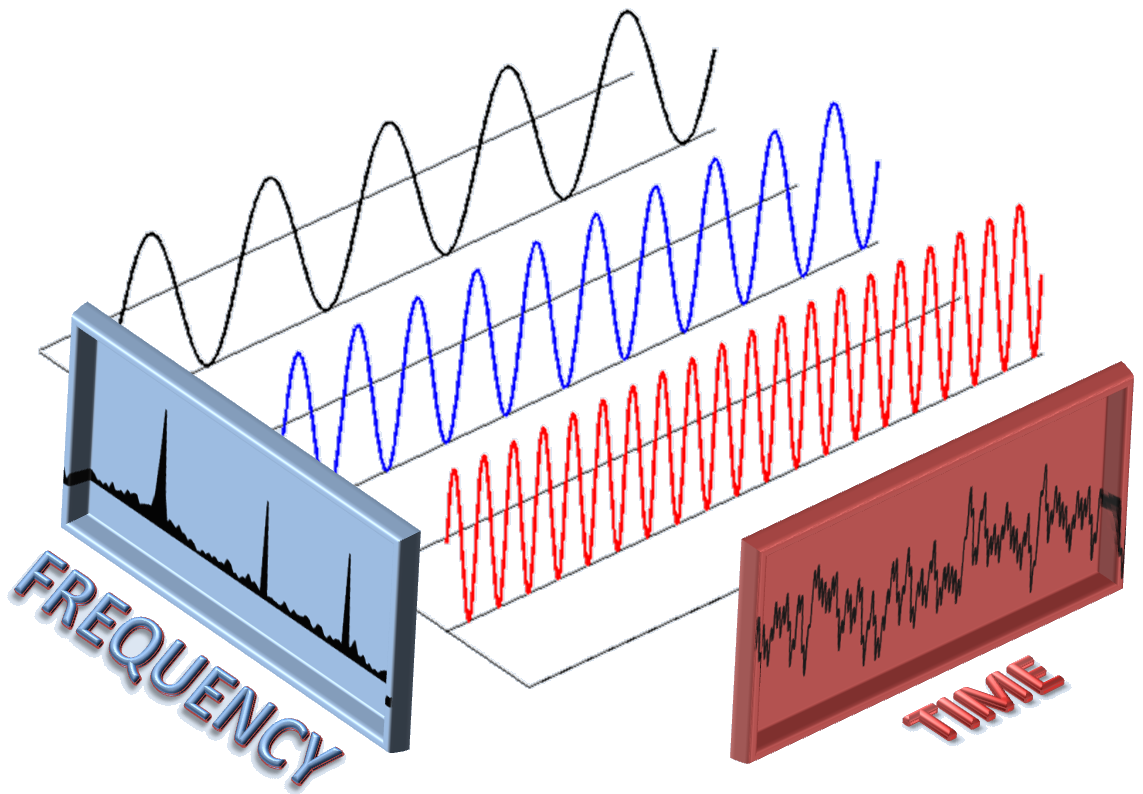
\includegraphics[scale=0.4]{title2.png}
		
		\vfill
		
		{\large \monthyear\today}
		
	\end{center}
\end{titlepage}
	
	\pagestyle{scrheadings}
	
	\chapter*{Ringraziamenti}
	La lista per esteso delle persone che dovrei ringraziare alla fine di questo percorso sarebbe veramente lunga: molti mi hanno aiutato e supportato, anche con il pi� piccolo dei gesti.\\
	Ringrazio la mia famiglia ed i miei amici, per aver creduto in me ed avermi spronato ad andare sempre avanti. Ringrazio la mia ragazza, Sara, per avermi sopportato ogni volta che ero in crisi riguardo all'Universit�.\\
	Infine, vorrei fare un ringraziamento speciale a mia sorella, Melissa, per l'aiuto e i consigli che mi ha dato, e per tutto il tempo che mi ha dedicato.\\
	Grazie.
	
	\tableofcontents
	\listoffigures
	
	\chapter*{Introduzione}
	\pagenumbering{arabic}
	\addcontentsline{toc}{chapter}{Introduzione}
	Gli ultimi 20 anni sono stati caratterizzati da un utilizzo sempre pi� frequente delle tecniche di visualizzazione di algoritmi, da parte dei docenti e di Informatica, dal momento che esse costituiscono un importante strumento per l'apprendimento e la comprensione dei pi� svariati tipi di algoritmo.\\
	Un altro strumento altrettanto importante, per i fini sopra indicati, � rappresentato dal Web. Sono infatti moltissime le applicazioni che permettono, a studenti e ricercatori di tutto il mondo, di scambiarsi e condividere dati e informazioni tramite Internet, facilitandone cos� l'apprendimento e la comprensione, affidandosi anche a strumenti multimediali come la produzione di un'immagine o di un video.\\
	\\
	Il progetto \textit{AlViE4} (\textit{Algorithm Visualization Environment}, ovvero \textit{Ambiente per la Visualizzazione di Algoritmi}) nasce appunto con l'intento di far incontrare queste due realt�, estendendo il programma \textit{AlViE}, per la visualizzazione di algoritmi, al mondo del Web, tramite le nuove possibilit� offerte dallo standard \textit{HTML5}.\\
	\\
	Questo lavoro si compone di quattro capitoli. Nel Capitolo \ref{chap:visualizzazioneAlgoritmi}, per cominciare, effettueremo una panoramica sulle tecniche di visualizzazione esistenti, soffermandosi in particolare sulla loro storia ed evoluzione. Inoltre, verr� proposta una tassonomia per la classificazione ed una maggior comprensione dei sistemi di visualizzazione di algoritmi.\\
	Parleremo poi, nel secondo Capitolo, dello standard \textit{HTML5} (\textit{HyperText Markup Language}, ovvero \textit{Linguaggio di Marcatura degli Ipertesti}): le novit� introdotte rispetto alla versione precedente, le caratteristiche principali e le motivazioni che ci hanno spinto a scegliere gli strumenti messi a disposizione da questo nuovo standard per l'estensione di \textit{AlViE} al mondo del Web.\\
	All'interno del Capitolo \ref{chap:alvie} analizzeremo nello specifico il funzionamento del sistema AlViE, indicandone le novit� introdotte nella quarta versione. Verr� fornito, in conclusione del Capitolo, un esempio passo-passo su come costruire un algoritmo interpretabile da AlViE, producendone quindi una visualizzazione.\\
	In conclusione, vedremo come � stato svolto il lavoro di estensione di AlViE al Web, indicando le tecniche di programmazione utilizzate ed i problemi riscontrati in fase di sviluppo.
	\chapter{Errori ed aritmetica finita}
	\label{chapterErroriAritmeticaFinita}
	\pagenumbering{arabic}
	\minitoc \mtcskip
	\lettrine{Q}{}uando si utilizza un metodo numerico per risolvere un problema matematico non sempre si ottiene un \textbf{risultato esatto}, ma un \textbf{risultato approssimato}, che differisce dal risultato esatto.\\
	Sia $x \in \mathbb{R}$ il risultato esatto e $\tilde{x}$ il risultato approssimato corrispondente \begin{defi}
		La quantit�
		$$ \Delta x \equiv \tilde{x} - x $$
		rappresenta l'\textbf{errore assoluto} commesso.
	\end{defi}
	Tuttavia questa quantit� non � un buon indice di valutazione dell'errore, in quanto l'errore non viene in alcun modo rapportato all'ordine di grandezza del risultato: un errore assoluto pari a $10^{-3}$ rappresenta un errore trascurabile se, ad esempio, $x = 10^{8}$ ma allo stesso tempo � un errore enorme per $x = 10^{-3}$.\\
	Per poter meglio valutare il ``peso'' che l'errore ha sul risultato approssimato viene quindi introdotto un nuovo concetto
	\begin{defi}
		Se $x \neq 0$, si dice \textbf{errore relativo} la quantit�
		$$\varepsilon_x \equiv \dfrac{\Delta x}{x} = \dfrac{\tilde{x} - x}{x}$$
	\end{defi}
	Spesso l'errore relativo viene rapportato ad 1: valori di $\varepsilon_x$ vicini a 0 significano un errore ``piccolo'', mentre un errore relativo pari ad 1 implica una perdita totale di informazione.\\	
	Le cause che portano al verificarsi di tale errore sul risultato sono principalmente tre:
	\begin{itemize}
		\item errori di discretizzazione, o troncamento;
		\item errori di convergenza;
		\item errori di \textit{round-off}.
	\end{itemize}
	
	\section{Errori di discretizzazione}
		Si ha un errore di \textbf{discretizzazione}, o di \textbf{troncamento}, quando il problema dato viene formulato nel continuo e, per poter definire un metodo numerico che lo risolva eseguibile su calcolatore, � necessario sostituire tale problema con uno discreto che lo approssimi.
		
	\section{Errori di convergenza}
		\label{sez1.2}
		Se un metodo numerico utilizza una \textbf{funzione d'iterazione} $\Phi (x)$, allora si dice che il metodo � di tipo \textbf{iterativo}: esso non fornisce direttamente la soluzione al problema, ma genera una successione di risultati intermedi $\{x_n\}$, definita da
		\begin{equation}\label{iter}x_{n+1} = \Phi (x_n),\quad n=0, 1, 2, \dots,\end{equation}
		con $x_0$ \textit{approssimazione iniziale} fissata, che converge alla soluzione $x^*$, ovvero
		\begin{equation}\label{conv}\lim_{x \to +\infty} x_n = x^*.\end{equation}
		� ovvio per� che un calcolatore non pu� eseguire infinite iterazioni, quindi sar� necessario definire un opportuno \textbf{criterio d'arresto}.
		\begin{defi}
			Se l'iterazione (\ref{iter}) viene arrestata a $n = N - 1$, utilizzando come risultato $x_N$ al posto di $x^*$, la quantit�
			$$x_N - x^*$$
			viene detta \textbf{errore assoluto di convergenza}.
		\end{defi}
		
	\section{Errori di \textit{round-off}}
		Si ha un \textbf{errore di round-off}, e pi� precisamente \textbf{di rappresentazione}, quando si tenta di rappresentare una quantit� numerica, che spesso ha bisogno di una quantit� infinita di informazione per essere rappresentata esattamente (come ad esempio i numeri irrazionali), su un calcolatore, che per forza di cose � costretto ad utilizzare un'\textit{aritmetica finita}.\\
		Quindi qualunque numero, in un calcolatore, viene rappresentato mediante una quantit� finita di informazione, dando luogo, appunto, agli \textit{errori di rappresentazione}.\\
		In un calcolatore, inoltre, ogni numero viene rappresentato utilizzando una \textit{notazione posizionale} che utilizza le potenza di una base fissata $b \in \mathbb{N}$, con $b \geq 2$.\\
		Quando si parla di \textit{errore di rappresentazione} si distinguono due casi:
		\begin{itemize}
			\item numeri interi;
			\item numeri reali.
		\end{itemize}
		
		\subsection{Numeri interi}
			Un numero intero viene rappresentato, con base $b \in \mathbb{N}$, mediante una stringa del tipo
			$$\alpha_0\alpha_1\dots\alpha_N,$$
			con
			$$\alpha_0 \in \{+, -\},\quad \alpha_i \in \{0,1,\dots,b-1\},\quad i=1,\dots,N.$$
			Questa stringa corrisponde al numero
			$$
				n =
				\begin{cases}
					\sum_{i=1}^{N}\alpha_ib^{N-i}, & \quad \text{se $\alpha_0=+$},\\
					\sum_{i=1}^{N}\alpha_ib^{N-i} - b^N, & \quad \text{se $\alpha_0=-$}.
				\end{cases}
			$$
			Quindi risulta che l'insieme dei numeri correttamente rappresentabili tramite questa rappresentazione �
			$$[-b^N, b^N -1].$$
			
		\subsection{Numeri reali}
			Fissata una base $b \in \mathbb{N}$, un numero reale viene rappresentato mediante una stringa del tipo
			\begin{equation}\label{stringaReale}\alpha_0\alpha_1\dots\alpha_m\beta_1\dots\beta_s,\end{equation}
			dove
			\begin{equation}\label{condStringaReale}\alpha_0 \in \{+,-\},\quad\alpha_i,\beta_j\in\{0,1,\dots,b-1\},\quad i=1,\dots,m,\quad j=1,\dots,s,\end{equation}
			e tale che
			$$\alpha_1 \neq 0,$$
			cio� tale che il numero sia normalizzato. Questa rappresentazione viene detta \textbf{rappresentazione scientifica normalizzata} in base \textit{b}.\\
			Fissato lo \textbf{shift} $\nu\in\mathbb{N}$, la stringa (\ref{stringaReale}) rappresenta il numero
			\begin{equation}
				\label{numReale}
				r = 
				\begin{cases}
					\rho b^{\eta} & \quad \text{se $\alpha_0 = +$,}\\
					-\rho b^{\eta} & \quad \text{se $\alpha_0 = -$.}
				\end{cases}
			\end{equation}
			dove $\rho$ e $\eta$, rispettivamente \textbf{mantissa} ed \textbf{esponente}, sono le quantit�
			$$\rho=\pm\sum_{i=1}^{m}\alpha_ib^{1-i},\qquad \eta=\left(\sum_{j=1}^{s}\beta_jb^{s-j}\right) -\nu.$$
			Talvolta viene chiamato esponente anche la sola quantit� $e=\sum_{j=1}^{s}\beta_jb^{s-j}$, ovvero la quantit� tale che $\eta=e-\nu$.
			\begin{defi}
				L'\textbf{insieme dei numeri di macchina}, o numeri \textit{floating-point}, � definito come
				$$\mathcal{M}=\{0\}\cup\{\text{numeri della forma (\ref{stringaReale})}\}.$$
			\end{defi}
			\begin{teo}
				\label{teor1.1}
				$\mathcal{M}$ ha un numero finito di elementi.
			\end{teo}
			\begin{teo}
				Per ogni numero reale della forma (\ref{numReale}) vale
				$$1\leq |\rho| < b.$$
			\end{teo}
			\begin{teo}
				\label{teor1.3}
				Il pi� piccolo ed il pi� grande (in valore assoluto), tra i numeri di macchina diversi da 0, sono rispettivamente dati da:
				\begin{align}
					\label{rMinMax}
					&r_{min}=b^{-\nu},\\
					&r_{max}=(1-b^{-m})b^{\varphi},\quad \varphi=b^s-\nu.
				\end{align}
			\end{teo}
			Solitamente lo \textit{shift} $\nu$ viene scelto in modo che $r_{min} \approx r_{max}^{-1}$, ovvero $\nu\approx\sfrac{b^s}{2}$.\\
			Risulta allora che i numeri di macchina appartengono all'insieme
			\begin{equation}\label{insI}\mathcal{I}=[-r_{max}, -r_{min}]\cup\{0\}\cup[r_{min}, r_{max}],\end{equation}
			che ha un numero infinito di elementi, mentre, per il Teorema \ref{teor1.1}, $\mathcal{M}$ ha un numero finito di elementi.\\
			Quindi si definisce una funzione
			$$fl:\mathcal{I}\rightarrow\mathcal{M},$$
			che associa numeri reali $x\in\mathcal{I}$ a numeri di macchina $fl(x)\in\mathcal{M}.$ Quando $x\neq fl(x)$ si commette un \textit{errore di rappresentazione}.\\
			Sia
			$$x=(\alpha_1.\alpha_2\dots\alpha_m\alpha_{m+1}\dots)b^{\eta}$$
			un elemento positivo di $\mathcal{I}$. � possibile rappresentare tale numero
			\begin{itemize}
				\item con troncamento
					$$fl(x)=(\alpha_1.\alpha_2\dots\alpha_m)b^{\eta};$$
				\item con arrotondamento
					$$fl(x)=(\alpha_1.\alpha_2\dots\alpha_{m-1}\tilde{\alpha}_m)b^{\eta},$$
					con
					$$
						\tilde{\alpha}_m =
						\begin{cases}
							\alpha_m, &\quad \text{se $\alpha_{m+1}<\sfrac{b}{2}$,}\\
							\alpha_m+1, &\quad \text{se $\alpha_{m+1}\geq\sfrac{b}{2}$,}
						\end{cases}
					$$
					con eventuali riporti sulle cifre precedenti alla \textit{m}-esima nel caso in cui $\tilde{\alpha}_m\geq b.$
			\end{itemize}
			Infine si impone che $fl(0)=0$ e che $fl(x)=-fl(-x)$, se $x\in\mathcal{I}$ ed $x<0$.
			\begin{teo}
				\label{teor1.4}
				Se $x\in\mathcal{I}$ e $x\neq 0$, allora
				$$fl(x)=x(1+\varepsilon_x),\quad |\varepsilon_x|\leq u,$$
				dove
				$$
					u =
					\begin{cases}
						b^{1-m}, &\quad \text{con troncamento},\\
						\dfrac{1}{2}b^{1-m}, &\quad \text{con arrotondamento}.
					\end{cases}
				$$
			\end{teo}
			\begin{defi}
				La quantit� \textit{u}, definita nel Teorema \ref{teor1.4}, � detta \textbf{precisione di macchina}.
			\end{defi}
			
		\subsection{\textit{Overflow} e \textit{Underflow}}
			Quando si cerca di rappresentare un numero reale non contenuto nell'insieme $\mathcal{I}$ definito nella (\ref{insI}) si incorre in particolari tipi di errori:
			\begin{itemize}
				\item se $|x|>r_{max}$\\
					allora l'errore viene chiamato \textbf{overflow} e spesso viene risolto rappresentando i numeri pi� alti in valore assoluto di $r_{max}$ come una quantit� infinita.
				\item se $0<|x|<r_{min}$\\
					si incorre in una condizione d'errore denominata di \textbf{underflow}. Si pu� risolvere o con la tecnica di \textbf{store 0}, che prevede di rappresentare questi numeri con uno 0, o con la tecnica denominata \textbf{gradual underflow}, che consiste nel denormalizzare la mantissa, includendo quindi nell'insieme $\mathcal{M}$ anche i \textit{numeri di macchina denormalizzati}.
			\end{itemize}
			Riassumendo l'implementazione della funzione $fl$ si ha che
			$$
				fl(x)=
				\begin{cases}
					0,&\quad \text{se $x=0$,}\\
					\tilde{x}\equiv x(1+\varepsilon_x),\quad |\varepsilon_x|\leq u,&\quad \text{se $r_{min}\leq |x|\leq r_{max}$,}\\
					underflow,&\quad \text{se $0<|x|<r_{min}$,}\\
					overflow,&\quad \text{se $|x|>r_{max}$.}
				\end{cases}
			$$
			
		\subsection{Lo standard IEEE 754}
			\label{subSec1.3.4}
			Lo standard per la rappresentazione di numeri reali pi� diffuso � l'\textit{IEEE 754}, che utilizza una reppresentazione in base $b=2$ ed utilizza una tecnica di arrotondamento definita \textbf{round to even}, ovvero rappresentando $fl(x)$ come il numero di macchina ``pi� vicino'' ad $x$ (nel caso vi fossero due numeri reali equidistanti viene scelto quello il cui ultimo bit della mantissa � \textit{pari}, ossia 0).\\
			Con questo standard viene guadagnato un bit della mantissa in quanto essa sar� sempre della forma $1.f$, per numeri normalizzati, o della forma $0.f$ per numeri denormalizzati. pertanto viene memorizzata soltanto la \textit{frazione} $f$.\\
			Lo standard si suddivide in due formati: \textit{singola precisione} e \textit{doppia precisione}.\\
			Di seguito � riportato il numero di bit assegnato a ciascun formato\\
			\begin{center}
				\begin{tabular}{c||c|c}
					& Singola precisione & Doppia precisione\\
					\hline
					segno & 1 & 1\\
					\hline
					frazione (mantissa) & 23 (24) & 52 (53)\\
					\hline
					esponente & 8 & 11\\
					\hline
					totale & 32 & 64\\
					\hline
				\end{tabular}
			\end{center}
			Mentre per quanto riguarda l'implementazione dei due formati si ha la seguente tabella:
			\begin{center}
				\begin{tabular}{|c|c|c|}
					\hline
					Singola & Doppia & \multirow{2}{*}{Interpretazione}\\
					precisione & precisione &\\
					\hline
					\multirow{2}{*}{$0<e<255$} & \multirow{2}{*}{$0<e<2047$} & mantissa normalizzata\\
					& & ($\nu=127$ in singola precisione, $\nu=1023$ in doppia)\\
					\hline
					\multicolumn{2}{|c|}{\multirow{2}{*}{$e=0$ e $f\neq 0$}} & mantissa denormalizzata\\
					\multicolumn{2}{|c|}{} & ($\nu=126$ in singola precisione, $\nu=1022$ in doppia)\\
					\hline
					\multicolumn{2}{|c|}{\multirow{2}{*}{$e=f=0$}} & zero\\
					\multicolumn{2}{|c|}{} & (con segno)\\
					\hline
					\multicolumn{2}{|c|}{$f=0$} & infinito\\
					$e=255$ & $e=2047$ & (con segno)\\
					\hline
					\multicolumn{2}{|c|}{$f\neq 0$} & NaN\\
					$e=255$ & $e=2047$ & (Not a Number)\\
					\hline
				\end{tabular}
			\end{center}
			
		\subsection{Aritmetica finita}
			Quando si eseguono delle operazioni in aritmetica finita si deve tenere conto dell'insieme di rappresentabilit�.\\
			Per quanto riguarda i numeri interi, se entrambi gli operandi ricadono nell'insieme di rappresentabilit�, allora l'implementazione non differisce dalla corrispettiva operazione algebrica.\\
			Se invece si sta operando con numeri reali, allora si deve tener conto che l'implementazione opera tra numeri di macchina e restituisce un numero di macchina come risultato.\\
			Ad esempio l'implementazione della somma algebrica in aritmetica finita sar�:
			\begin{equation}\label{sommaAF}x\oplus y = fl(fl(x) + fl(y),\quad x,y\in\mathbb{R}.\end{equation}
			Ovviamente, in questo secondo caso, propriet� come associativit� o distributivit� possono non valere pi�.\\
			
		\subsection{Conversione tra tipi diversi}
			Spesso capita di dover convertire un numero intero in un reale e viceversa. La conversione da intero a reale � sempre possibile, introducendo al pi� un errore dell'ordine di $u$, se il numero di bit della mantissa non bastano a rappresentare il numero (a parit� di bit nella rappresentazione come intero e come reale si ha che la mantissa ha meno bit a disposizione rispetto alla rappresentazione come intero). La conversione da reale ad intero � invece, generalmente, pi� problematica, in quanto il numero che si vuole convertire potrebbe non appartenere all'insieme degli interi rappresentabili $\{-b^N,\dots ,b^N-1\}$, come ad esempio tutti i numeri con virgola.
		
	\section{Condizionamento di un problema}
		\label{sez1.4}
		Sia
		\begin{equation}\label{problDef}y=f(x)\end{equation}
		la formalizzazione di un problema matematico che vogliamo risolvere, con $x\in\mathbb{R}$ dati di ingresso, $f:\mathbb{R}\rightarrow\mathbb{R}$ funzione che descrive formalmente il problema ed $y\in\mathbb{R}$ soluzione del problema.\\
		Quando si decide di risolvere un problema del genere con un calcolatore viene definito un opportuno metodo numerico che risolva il problema in questione, ma di fatto il problema che ci troveremo a risolvere sar� del tipo
		$$\tilde{y}=\tilde{f}(\tilde{x}),$$
		dove $\tilde{x}$ rappresenta i dati in ingresso \textit{perturbati} (cio� con errori di \textit{round-off} o ottenuti sperimentalmente), $\tilde{f}$ indica che il metodo numerico � implementato in aritmetica finita (con eventuali errori di \textit{discretizzazione} o \textit{convergenza}) e $\tilde{y}$ denota i dati in uscita affetti dai precedenti errori.\\
		Ci� che � interessante studiare � il \textbf{condizionamento del problema}, ovvero come gli errori sui dati in ingresso $\varepsilon_x=\dfrac{\tilde{x}-x}{x}$ si propagano attraverso l'esecuzione del metodo numerico fino a definire l'errore $\varepsilon_y=\dfrac{\tilde{y}-y}{y}$ commesso sulla soluzione finale. Per un'analisi pi� approfondita e completa dell'errore del metodo numerico utilizzato si dovrebbero considerare anche gli errori introdotti dall'utilizzo di $\tilde{f}$ al posto di $f$, tuttavia, per semplicit�, ci limitiamo a studiare il problema
		$$\tilde{y}=f(\tilde{x}).$$
		Come accennato precedentemente, se si considerano gli errori relativi sui dati di ingresso e sulla soluzione finale si ha che
		$$\tilde{x}=x(1+\varepsilon_x),\quad\tilde{y}=y(1+\varepsilon_y).$$
		Ci� che ci interessa determinare �, quindi, la relazione che intercorre tra $\varepsilon_x$ e $\varepsilon_y$.\\
		Sviluppando $f(\tilde{x})$ in $x$ si ottiene
		$$f(\tilde{x})=f(x(1+\varepsilon_x))=f(x+x\varepsilon_x)=P_1(x+x\varepsilon_x;x)+O((x\varepsilon_x)^2)=f(x)+f'(x)x\varepsilon_x+O(\varepsilon_x^2),$$
		ovvero
		$$\tilde{y}=y-y\varepsilon_y = f(x)+f'(x)x\varepsilon_x+O(\varepsilon_x^2).$$
		Ricordando la (\ref{problDef}) e considerando un'\textit{analisi al primo ordine} (ovvero trascurando l'errore $O(\varepsilon_x^2)$), si ha che
		$$y+y\varepsilon_y\approx y+f'(x)x\varepsilon_x$$
		$$y\varepsilon_y\approx f'(x)x\varepsilon_x$$
		$$\varepsilon_y\approx f'(x)\dfrac{x}{y}\varepsilon_x$$
		$$|\varepsilon_y|\approx |f'(x)\dfrac{x}{y}|\cdot |\varepsilon_x| \equiv k|\varepsilon_x|.$$
		Quindi si ha che
		\begin{equation}\label{numCond}k \equiv |f'(x)\dfrac{x}{y}|.\end{equation}
		\begin{defi}
			Il \textit{fattore di amplificazione} $k$, che misura di quanto gli errori sui dati iniziali si possono amplificare sull'errore della soluzione finale, � detto \textbf{numero di condizionamento del problema} (\ref{problDef}).
		\end{defi}
		L'ordine di grandezza di $k$ determina quindi il condizionamento del problema:
		\begin{itemize}
			\item se $k\approx 1$, allora l'ordine degli errori finali � uguale a quello degli errori sui dati in ingresso ed il problema si dice \textbf{ben condizionato}.
			\item se $k\gg 1$ significa che nell'eseguire il metodo numerico gli errori finali risultano essere molto pi� grandi rispetto agli errori sui dati in ingresso. Il problema si dice in questo caso \textbf{malcondizionato}.
		\end{itemize}
		Se un problema risulta avere numero di condizionamento pari a $k\approx u^{-1}$, allora qualunque risultato sar� privo di significato: infatti l'errore sui dati di ingresso sar� dell'ordine di $u$, il che vuol dire che risulter� $\varepsilon_y=1$, che equivale ad una totale perdita di informazione. Se il problema risulta essere malcondizionato l'unica possibilit� per ottenere risultati accettabili � quella di riformulare il problema tentando di ottenere un condizionamento migliore; se invece il problema � ben condizionato si deve utilizzare un metodo numerico che risolva il problema mantenendone le buone propriet� di condizionamento (tali metodi numerici sono detti \textit{metodi numericamente stabili}).\\
		Analizziamo il condizionamento delle operazioni algebriche elementari:
		\begin{itemize}
			\item \textbf{\underline{Somma algebrica}}\\
				Il problema in questione �
				$$y=x_1+x_2,\qquad x_1,x_2\in\mathbb{R},\quad x_1+x_2\neq 0.$$
				Siano $\varepsilon_1$ e $\varepsilon_2$ gli errori sui dati in ingresso, si ha
				$$y(1+\varepsilon_y)=x_1(1+\varepsilon_1)+x_2(1+\varepsilon_2)=x_1+x_2+x_1\varepsilon_1+x_2\varepsilon_2.$$
				Si ottiene quindi
				$$y\varepsilon_y=x_1+x_2+x_1\varepsilon_1+x_2\varepsilon_2 -y$$
				$$y\varepsilon_y=x_1+x_2+x_1\varepsilon_1+x_2\varepsilon_2 -x_1-x_2$$
				$$|y\varepsilon_y|=|x_1\varepsilon_1+x_2\varepsilon_2|\leq |x_1\varepsilon_1|+|x_2\varepsilon_2|\leq (|x_1|+|x_2|)\varepsilon_x,\quad\varepsilon_x=max\{|\varepsilon_1|,|\varepsilon_2|\}$$
				\begin{equation}\label{condSomma}|\varepsilon_y|\leq\dfrac{|x_1|+|x_2|}{|y|}\varepsilon_x=\dfrac{|x_1|+|x_2|}{|x_1+x_2|}\varepsilon_x.\end{equation}
				Quindi risulta che
				$$k\leq\dfrac{|x_1|+|x_2|}{|x_1+x_2|}.$$
				Detto questo si possono avere due casi:
				\begin{itemize}
					\item $x_1x_2>0$: se gli addendi sono concordi, allora $k=1$ e la somma � ben condizionata;
					\item $x_1\approx -x_2$: se invece gli addendi sono di segno opposto il numero di condizionamento $k$ pu� essere arbitrariamente grande, perci� in questo caso la somma � malcondizionata. Questo particolare malcondizionamento, in aritmetica finita, prende il nome di \textit{cancellazione numerica}.
				\end{itemize}
			\item \textbf{\underline{Moltiplicazione}}\\
				Il problema della moltiplicazione di due numeri reali � formulato come segue:
				$$y=x_1x_2,\qquad x_1,x_2\in\mathbb{R},\quad x_1x_2\neq 0$$
				Introducendo gli errori relativi
				$$y(1+\varepsilon_y)=x_1(1+\varepsilon_1)x_2(1+\varepsilon_2)=x_1x_2(1+\varepsilon_1+\varepsilon_2+\varepsilon_1\varepsilon_2).$$
				Trascurando il termine quadratico si ha che
				\begin{align*}
					y\varepsilon_y&\approx x_1x_2(1+\varepsilon_1+\varepsilon_2)-y=\\
					&=x_1x_2(1+\varepsilon_1+\varepsilon_2)-x_1x_2=\\
					&=x_1x_2(\varepsilon_1+\varepsilon_2)
				\end{align*}
				$$\varepsilon_y\approx\dfrac{x_1x_2(\varepsilon_1+\varepsilon_2)}{x_1x_2}=\varepsilon_1+\varepsilon_2$$
				$$|\varepsilon_y|\approx |\varepsilon_1+\varepsilon_2|\leq 2\varepsilon_x,\qquad \varepsilon_x=\{|\varepsilon_1|, |\varepsilon_2|\}.$$
				Quindi il numero di condizionamento risulta essere $k=2$, pertanto la moltiplicazione � sempre ben condizionata.
			\item \textbf{\underline{Divisione}}\\
				Esaminiamo adesso il problema
				$$y=\dfrac{x_1}{x_2},\qquad x_1,x_2\in\mathbb{R},\quad x_1x_2\neq 0.$$
				Si ha che
				\begin{align*}
					y(1+\varepsilon_y)&=\dfrac{x_1(1+\varepsilon_1)}{x_2(1+\varepsilon_2)}=\dfrac{x_1}{x_2}\cdot\dfrac{(1+\varepsilon_1)(1-\varepsilon_2)}{(1+\varepsilon_2)(1-\varepsilon_2)}=\dfrac{x_1}{x_2}\cdot\dfrac{(1+\varepsilon_1)(1-\varepsilon_2)}{(1-\varepsilon_2^2)}\approx\\
					&\approx \dfrac{x_1}{x_2}(1+\varepsilon_1)(1-\varepsilon_2)=\dfrac{x_1}{x_2}(1+\varepsilon_1-\varepsilon_2-\varepsilon_1\varepsilon_2),
				\end{align*}
				dove l'approssimazione � dovuta al fatto che si � trascurato il termine quadratico $\varepsilon_2^2$.\\
				Trascurando anche il termine quadratico $\varepsilon_1\varepsilon_2$ si ottiene quindi
				$$y\varepsilon_y\approx\dfrac{x_1}{x_2}(1+\varepsilon_1-\varepsilon_2)-y$$
				$$y\varepsilon_y\approx\dfrac{x_1}{x_2}(1+\varepsilon_1-\varepsilon_2)-\dfrac{x_1}{x_2}$$
				$$\varepsilon_y\approx\dfrac{x_1}{x_2}(\varepsilon_1-\varepsilon_2)\cdot\dfrac{x_2}{x_1}$$
				$$\varepsilon_y\approx\varepsilon_1-\varepsilon_2$$
				$$|\varepsilon_y|\approx|\varepsilon_1-\varepsilon_2|\leq 2\varepsilon_x,\qquad\varepsilon_x=\{|\varepsilon_1|,|\varepsilon_2|\}.$$
				Anche in questo caso il numero di condizionamento del problema risulta essere $k=2$, quindi la divisione, come la moltiplicazione, � sempre ben condizionata.
		\end{itemize}
		
	\section*{Esercizi}
		\addcontentsline{toc}{section}{Esercizi}
		\markboth{\textsc{\uppercase{Capitolo }\ref{chapterErroriAritmeticaFinita}\uppercase{. Errori ed aritmetica finita}}}{\textsc{\uppercase{Esercizi}}}
		\begin{es} %1.1
			\label{es:1.1}
			Sia $x = \pi \approx 3.1415 = \tilde{x}$. Calcolare il corrispondente errore relativo $\varepsilon_x$. Verificare che il numero di cifre decimali corrette nella rappresentazione approssimata di $x$ mediante $\tilde{x}$ � all'incirca dato da
			$$-\log_{10} |\varepsilon_x|.$$
		\end{es}
		\begin{sol}
			Per definizione di errore relativo si ha che
			$$\varepsilon_x = \dfrac{\tilde{x} - x}{x} = \dfrac{3.1415 - \pi}{pi} \approx -2.9493 \times 10^{-5}$$
			Risulta allora che $-\log_{10}|\varepsilon_x| \approx 4.5303$; infatti 4 � il numero di cifre decimali esatte di 3.1415 come approssimazione di $\pi$ in quanto l'errore assoluto
			$$\Delta x = \tilde{x} - x = 3.1415 - \pi \approx -9.2654 \times 10^{-5}$$
			risulta essere dell'ordine di $10^{-5}$, ovvero ha le prime 4 cifre decimali pari a zero.
			\begin{flushright}
				\underline{Riferimenti \textsc{Matlab}}\\
				Codice \ref{lst:es1.1} (pagina \pageref{lst:es1.1})
			\end{flushright}
		\end{sol}
		\sectionline
		\begin{es} %1.2
			Dimostrare che, se $f(x)$ � sufficientemente regolare e $h > 0$ � una quantit� ``piccola'', allora:
			$$\dfrac{f(x_0 + h) - f(x_0 - h)}{2h} = f'(x_0) + O(h^2),$$
			$$\dfrac{f(x_0 + h) -2f(x_0) + f(x_0 - h)}{h^2} = f''(x_0) + O(h^2).$$
		\end{es}
		\begin{sol}
			Per queste due dimostrazioni si deve sviluppare la funzione $f(x)$ mediante un polinomio di Taylor di grado opportuno. Ricordiamo che lo sviluppo in polinomio di Taylor di grado \textit{n} della funzione $f(x)$ centrato in $x_0$ � $P_n(x; x_0) = \sum_{k=0}^{n} \dfrac{(x - x_0)^k}{k!}f^{(k})(x_0)$ e che il resto \textit{n}-esimo vale $R_n(x; x_0) = O(x - x_0)^{n+1}$.\\
			Per la prima uguaglianza si sviluppa $f(x)$ nel polinomio di Taylor al secondo ordine
			\begin{align*}
				f(x) &= P_2(x;x_0)+R_2(x;x_0)=\\
				&=f(x_0) + (x - x_0)f'(x_0) + \dfrac{(x - x_0)^2}{2}f''(x_0) + O((x - x_0)^3).
			\end{align*}
			Calcolando questo sviluppo in $x = (x_0 + h)$ e $x = (x_0 - h)$ si ottiene
			$$f(x_0 + h) = f(x_0) +hf'(x_0) + \dfrac{h^2}{2}f''(x_0) + O(h^3),$$
			$$f(x_0 - h) = f(x_0) -hf'(x_0) + \dfrac{h^2}{2}f''(x_0) + O(h^3).$$
			Quindi sostituendo nel rapporto incrementale di partenza si ha che
			\begin{align*}
				\dfrac{f(x_0 + h) - f(x_0 - h)}{2h} &= \dfrac{f(x_0) + hf'(x_0) + \dfrac{h^2}{2}f''(x_0) + O(h^3)}{2h} +\\
				&-\dfrac{f(x_0) - hf'(x_0) + \dfrac{h^2}{2}f''(x_0) + O(h^3)}{2h} =\\
				&=\dfrac{2hf'(x_0) + o(h^3)}{2h} = f'(x_0) + O(h^2).
			\end{align*}
			Per la seconda uguaglianza � invece necessario utilizzare un'approssimazione con Taylor al terzo ordine
			\begin{align*}
			f(x) &= P_3(x;x_0)+R_3(x;x_0)=\\
			&=f(x_0) + (x - x_0)f'(x_0) + \dfrac{(x - x_0)^2}{2}f''(x_0) +\\
			&+ \dfrac{(x - x_0)^3}{6}f'''(x_0) + O((x - x_0)^4)
			\end{align*}
			e come prima si calcola tale sviluppo in $x = (x_0 + h)$ e $x = (x_0 - h)$
			$$f(x_0 + h) = f(x_0) + hf'(x_0) + \dfrac{h^2}{2}f''(x_0) + \dfrac{h^3}{6}f'''(x_0) + O(h^4),$$
			$$f(x_0 - h) = f(x_0) - hf'(x_0) + \dfrac{h^2}{2}f''(x_0) - \dfrac{h^3}{6}f'''(x_0) + O(h^4).$$
			Quindi sostituendo come nell'uguaglianza precedente si ottiene
			\begin{align*}
				\dfrac{f(x_0 + h) -2f(x_0) + f(x_0 - h)}{h^2} &= \dfrac{h^2f''(x_0) + O(h^4)}{h^2} =\\
				&= f''(x_0) + O(h^2).
			\end{align*}
		\end{sol}
		\sectionline
		\begin{es} %1.3
			\label{es:1.3}
			Dimostrare che il metodo iterativo (\ref{iter}), convergente a $x^*$ (vedi (\ref{conv})), deve verificare la condizione di consistenza
			$$x^* = \Phi (x^*).$$
			Ovvero, la soluzione cercata deve essere un \underline{punto fisso} per la funzione di iterazione che definisce il metodo.
		\end{es}
		\begin{sol}
			Essendo il metodo iterativo convergente, per definizione risulta che
			$$\lim_{x \to +\infty} x_n = x^*.$$
			Supponendo la funzione $\Phi (x_n)$ continua, si ha
			$$\lim_{n \to +\infty} \Phi (x_n) = \Phi (\lim_{n \to +\infty} x_n) = \Phi (x^*),$$
			inoltre, essendo per definizione $\Phi (x_n) = x_{n+1}$,
			$$\lim_{n \to +\infty} \Phi (x_n) = \lim_{x \to +\infty} x_{n+1} = x^*,$$
			da cui la tesi, $x^* = \Phi (x^*).$
		\end{sol}
		\sectionline
		\begin{es} %1.4
			\label{es:1.4}
			Il metodo iterativo
			$$x_{n+1} = \dfrac{x_nx_{n+1} +2}{x_n +x_{n-1}},\quad n=1, 2,\dots,\quad x_0=2, x_1=1.5,$$
			definisce una successione di approssimazioni convergente a $\sqrt{2}$. Calcolare a quale valore si \textit{n} bisogna arrestare l'iterazione, per avere un errore di convergenza $\approx 10^{-12}$. Comparare con i risultati nella seguente tabella
			\begin{center}
				\begin{tabular}{|c|l|}
					\hline
					\textit{n} & $x_n$\\
					\hline
					0 & $2$\\
					1 & $1.5$\\
					2 & $1.416666666666\dots$\\
					3 & $1.414215686274\dots$\\
					4 & $1.414213562374\dots$\\
					\hline
				\end{tabular}
			\end{center}
			relativa all'iterazione
			$$x_{n+1} = \dfrac{1}{2}\left(x_n + \dfrac{2}{x_n}\right),\quad n=0,1,2,\dots,\quad x_0=2.$$
			che approssima $\sqrt{2}.$
		\end{es}
		\begin{sol}
			Risulta che il primo metodo iterativo proposto (quello con i due punti iniziali $x_0$ ed $x_1$) approssima $\sqrt{2}$ con errore di convergenza assoluto dell'ordine di $10^{-12}$ per $i = 6$, come si pu� vedere dalla tabella seguente
			\begin{center}
				\begin{tabular}{c||l|l}
					\textit{i} & $x_i$ & $\Delta x$\\
					\hline
					0 & $2$ & $5.85786e-001$\\
					1 & $1.5$ & $8.57864e-002$\\
					2 & $1.428571428571\dots$ & $1.43578e-002$\\
					3 & $1.414634146341\dots$ & $4.20583e-004$\\
					4 & $1.414215686274\dots$ & $2.12390e-006$\\
					5 & $1.414213562688\dots$ & $3.15774e-010$\\
					6 & $1.414213562373\dots$ & $0$
				\end{tabular}
			\end{center}
			Per $i \geq 6$ l'errore riportato � 0, probabilmente a causa della precisione di macchina che non riesce a rappresentare numeri troppo ``piccoli''.\\
			Il secondo metodo proposto (quello con il solo punto iniziale $x_0 = 2$) risulta invece raggiungere un errore assoluto di convergenza per $i=4$.\\
			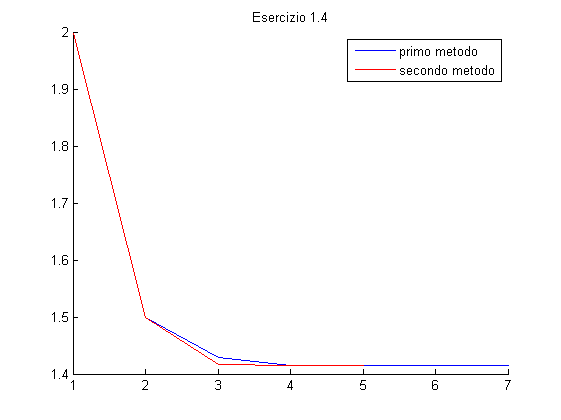
\includegraphics[width=0.8\textwidth]{es1_4.png}
			\begin{flushright}
				\underline{Riferimenti \textsc{Matlab}}\\
				Codice \ref{lst:es1.4} (pagina \pageref{lst:es1.4})
			\end{flushright}
		\end{sol}
		\sectionline
		\begin{es} %1.5
			Il codice Fortran
			\lstinputlisting[language=Fortran, frame=none, stepnumber=0, nolol=true]{code/fortran1_5.txt}
			produce il seguente output:
			\begin{center}
				\begin{tabular}{r r}
					1 & 32765\\
					2 & 32766\\
					3 & 32767\\
					4 & -32768\\
					5 & -32767\\
					6 & -32766\\
					7 & -32765\\
					8 & -32764\\
					9 & -32763\\
					10 & -32762
				\end{tabular}
			\end{center}
			Spiegarne il motivo.
		\end{es}
		\begin{sol}
			Essendo la variabile \textit{numero} di 2 byte significa che il bit pi� significativo ($\alpha_0$) rappresenta il segno (0 per un numero positivo ed 1 per un numero negativo), mentre i restanti 15 bit (da $\alpha_1$ ad $\alpha_15$) rappresentano il modulo del numero espresso in complemento a 2.\\
			Quando viene stampata la terza iterazione il numero vale 32767, ovvero
			$$\underbrace{0}_+\underbrace{111111111111111}_{32767},$$
			e ci si aspetta quindi che la quarta iterazione stampi il numero 32768. Tuttavia il numero 32768 avrebbe bisogno, per essere rappresentato in binario, di 16 bit per il modulo e di 1 per il segno, per un totale di 17. Infatti, eseguendo la somma in base due si ottiene
			$$\underbrace{1}_-\underbrace{000000000000000}_{32768},$$
			in quanto il riporto viene propagato fino al bit del segno.\\
			Successivamente il numero viene correttamente incrementato.
		\end{sol}
		\sectionline
		\begin{es} %1.6
			\label{es:1.6}
			Dimostrare i Teoremi \ref{teor1.1} e \ref{teor1.3}.
		\end{es}
		\begin{sol}
			\begin{itemize}
				\item \underline{Teorema \ref{teor1.1}}:\\
					Essendo l'insieme $\mathcal{M}$
					$$\mathcal{M}=\{0\}\cup\{\text{numeri della forma (\ref{stringaReale})}\},$$
					risulta che
					$$|\mathcal{M}|=|\{0\}|+|\{\text{numeri della forma (\ref{stringaReale})}\}|.$$
					Per la (\ref{condStringaReale}) si vede che:
					\begin{itemize}
						\item $\alpha_0$ pu� assumere 2 valori;
						\item $\alpha_1$ pu� assumere $b-1$ valori;
						\item $\alpha_i$, $\beta_j$ possono assumere \textit{b} valori, per $i=2,\dots,m$, $j=~1,\dots,s$.
					\end{itemize}
					Quindi la cardinalit� di $\mathcal{M}$ � data dalle disposizioni con ripetizione di questi elementi, ovvero
					$$|\mathcal{M}|=2(b-1)b^{m+s}+1<+\infty.$$
				\item \underline{Teorema \ref{teor1.3}}:\\
					Per quanto riguarda il minimo numero di macchina, positivo e diverso da 0, si ha che la mantissa minima vale $\rho_{min}=1$, mentre l'esponente minimo vale $\eta_{min}=0-\nu=-\nu$; quindi, applicando la (\ref{numReale})
					$$r_{min} = \rho_{min}b^{\eta_{min}} = 1\cdot b^{-\nu}=b^{-\nu}.$$
					Invece, per quanto riguarda $r_{max}$, si ha che la mantissa � massima quando tutti i suoi bit valgono $(b-1)$, ovvero
					\begin{align*}
						\rho_{max} &= (b-1)\sum_{i=1}^{m}b^{1-i} = (b-1)\sum_{k=0}^{m-1}b^{-k} =\\
						&=(b-1)\sum_{k=0}^{m-1}\left(\dfrac{1}{b}\right)^{k},
					\end{align*}
					ricordando che $\left(1-\dfrac{1}{b}\right)\sum_{k=0}^{m-1}\left(\dfrac{1}{b}\right)^k=1^m-\left(\dfrac{1}{b}\right)^m$, ovvero che $\sum_{k=0}^{m-1}\left(\dfrac{1}{b}\right)^k=b\dfrac{1-b^{-m}}{b-1}$, si ha che
					$$\rho_{max}=b\left(1-b^{-m}\right).$$
					Per quanto riguarda l'esponente massimo, risulta invece
					\begin{align*}
						\eta_{max}&=\left[(b-1)\sum_{i=1}^{s}b^{s-j}\right]-\nu=\left[(b-1)b^{s-1}\sum_{k=0}^{s-1}b^{-k}\right]-\nu=\\
						&=[b^s(1-b^{-s})]-\nu=(b^s-1)-\nu.
					\end{align*}
					Quindi, applicando di nuovo la (\ref{numReale}), si ottiene
					$$r_{max}=b\left(1-b^{-m}\right)b^{b^s-1-\nu} =\left(1-b^{-m}\right)b^{b^s-\nu}.$$
			\end{itemize}
		\end{sol}
		\sectionline
		\begin{es} %1.7
			Dimostrare il Teorema \ref{teor1.4} nel caso della rappresentazione con arrotondamento.
		\end{es}
		\begin{sol}
			Si distinguono i due casi in cui si ha arrotondamento per difetto e per eccesso:
			\begin{itemize}
				\item per difetto:\\
					In questo caso si ha che $\tilde{\alpha}_m=\alpha_m$ in quanto $\alpha_{m+1}<\sfrac{b}{2}$.
					\begin{align*}
						|\varepsilon_x|&=\dfrac{|x-fl(x)|}{|x|}=\dfrac{|(\alpha_1.\alpha_2\dots\alpha_m\alpha_{m+1}\dots-\alpha_1.\alpha_2\dots\tilde{\alpha}_m)b^{\eta}|}{|(\alpha_1.\alpha_2\dots)b^{\eta}|}=\\
						&=\dfrac{|0.\overbrace{0\dots0}^{m-1}\alpha_{m+1}\dots|}{|\alpha_1.\alpha_2\dots|},
					\end{align*}
					quindi, essendo il denominatore sicuramente $\geq 1$, il reciproco sar� sicuramente $\leq 1$. Se poi si trasla il numeratore di $m$ posizioni otteniamo
					$$|\varepsilon_x|\leq|(\alpha_{m+1}.\alpha_{m+2}\dots)b^{-m}|<\dfrac{b}{2}b^{-m}=\dfrac{1}{2}b^{1-m}\equiv u.$$
				\item per eccesso:\\
					In questo caso invece risulta che $\tilde{\alpha}_m=\alpha_m+1$, essendo $\alpha_{m+1}\geq\sfrac{b}{2}$.
					\begin{align*}
						|\varepsilon_x|&=\dfrac{|x-fl(x)|}{|x|}=\dfrac{|(\alpha_1.\alpha_2\dots\alpha_m\alpha_{m+1}\dots-\alpha_1.\alpha_2\dots\tilde{\alpha}_m)b^{\eta}|}{|(\alpha_1.\alpha_2\dots)b^{\eta}|}=\\
						&=\dfrac{|0.\overbrace{0\dots0}^{m-1}\hat{\alpha}_{m+1}\dots|}{|\alpha_1.\alpha_2\dots|},
					\end{align*}
					con $\hat{\alpha}_{m+1}=\tilde{\alpha}_m0-\alpha_m\alpha_{m+1}\leq\sfrac{b}{2}$.\\
					In questo caso per� � possibile che il valore assoluto al numeratore, traslato di $m$ posizioni, sia $>\sfrac{b}{2}$, come ad esempio nel caso estremo in cui $\hat{\alpha}_{m+1}=\sfrac{b}{2}$ e tutte le cifre successive valgono $(b-1)$. Quando si verifica questo si nota, tuttavia, che dividendo tale quantit� per il valore assoluto al denominatore si ottiene sicuramente una quantit� $<\sfrac{b}{2}$.\\
					Quando invece il valore assoluto al numeratore (traslato di $m$ posizioni) risulta gi� essere $\leq\sfrac{b}{2}$ si procede come nel caso precedente per difetto.\\
					Quindi in ogni caso si ha che
					$$|\varepsilon_x|\leq\dfrac{b}{2}b^{-m}=\dfrac{1}{2}b^{1-m}\equiv u.$$
			\end{itemize}
		\end{sol}
		\sectionline
		\begin{es} %1.8
			\label{es:1.8}
			Quante cifre binarie sono utilizzate per rappresentare, mediante arrotondamento, la mantissa di un numero, sapendo che la precisione di macchina � $u\approx 4.66\cdot 10^{-10}$?
		\end{es}
		\begin{sol}
			Applicando il Teorema \ref{teor1.4} si ha che $u=\dfrac{1}{2}b^{1-m}$, ovvero che
			$$m=1-\log_b2u.$$
			Ponendo $b=2$ e $u=4.66\cdot 10^{-10}$ e arrotondando, eventualmente, per eccesso, risulta
			$$m=-\log_24.66\cdot 10^{-10}\approx 31.$$
			Quindi servono almeno 31 cifre binarie per la mantissa per avere una precisione di macchina non superiore a $4.66\cdot 10^{-10}$.
			\begin{flushright}
				\underline{Riferimenti \textsc{Matlab}}\\
				Codice \ref{lst:es1.8} (pagina \pageref{lst:es1.8})
			\end{flushright}
		\end{sol}
		\sectionline
		\begin{es} %1.9
			Dimostrare che, detta $u$ la precisione di macchina utilizzata,
			$$-\log_{10}u$$
			fornisce, approssimativamente, il numero di cifre decimali correttamente rappresentate nella mantissa.
		\end{es}
		\begin{sol}
			Studiamo separatamente i casi in cui la rappresentazione avviene tramite troncamento e tramite arrotondamento.\\
			\begin{itemize}
				\item con troncamento:\\
					Per il Teorema \ref{teor1.4}, posto $b=10$, si ha che
					$$u=10^{1-m}\Rightarrow \log_{10}u=1-m\Rightarrow m=1-\log_{10}u\approx -\log_{10}u.$$
				\item con arrotondamento:\\
					Sempre per il Teorema \ref{teor1.4}, con $b=10$,
					\begin{align*}
						u&=\dfrac{1}{2}10^{1-m}\Rightarrow\log_{10}2u=1-m\Rightarrow\\
						&
						\begin{aligned}
							\Rightarrow m&=1-\log_{10}2u=1-\log_{10}2-\log_{10}u=\\
							&=\log_{10}5-\log_{10}u\approx -\log_{10}u.
						\end{aligned}
					\end{align*}
			\end{itemize}
		\end{sol}
		\sectionline
		\begin{es} %1.10
			\label{es:1.10}
			Con riferimento allo standard \textit{IEEE 754} (vedi Sezione \ref{subSec1.3.4}) determinare, relativamente alla doppia precisione:
			\begin{enumerate}
				\item il pi� grande numero di macchina,
				\item il pi� piccolo numero di macchina normalizzato positivo,
				\item il pi� piccolo numero di macchina denormalizzato positivo,
				\item la precisione di macchina.
			\end{enumerate}
			Confrontare le risposte ai primi due quesiti col risultato fornito dalle function \textsc{Matlab} \lstinline{realmax} e \lstinline{realmin}.
		\end{es}
		\begin{sol}
			\begin{enumerate}
				\item Si ha che il pi� grande numero di macchina in doppia precisione � dato dalla mantissa massima e l'esponente massimo. Per l'Esercizio \ref{es:1.6} si ha che $\rho=b(1-b^{-m})=2(1-2^{-53})=2-2^{-52}$, mentre $\eta=2046-\nu=2046-1023=1023$, essendo il valore $e=2047$ riservato.\\
					Quindi il massimo numero di macchina risulta essere
					$$r_{max}=(2-2^{-52})2^{1023}\approx 1.8\cdot 10^{308},$$
					infatti la function \lstinline{realmax} di \textsc{Matlab} restituisce lo stesso risultato.
				\item Per quanto riguarda il pi� piccolo numero di macchina normalizzato positivo basta applicare la (\ref{rMinMax}), con l'accortezza che l'esponente $e=0$ � riservato e quindi il pi� piccolo esponente risulta essere $e=1$:
					$$r_{minN}=2^{1-\nu}=2^{1-1023}=2^{-1022}\approx 2.2\cdot 10^{-308}.$$
					Utilizzando la function \textsc{Matlab} \lstinline{realmin} si perviene allo stesso risultato.
				\item Il pi� piccolo numero di macchina denormalizzato positivo � caratterizzato, per definizione, dall'esponente $e=0$ e dalla mantissa minima diversa da 0, ovvero la mantissa che ha tutti i bit, tranne il meno significativo, a 0, che vale $\rho=2^{-52}$.\\
					Quindi
					$$r_{minD}=2^{-52}2^{0-\nu}=2^{-52}2^{-1022}\approx 4.9\cdot 10^{-324}.$$
				\item Dal momento che lo standard \textit{IEEE 754} utilizza la rappresentazione con arrotondamento, per il Teorema \ref{teor1.4} si ha
					$$u=\dfrac{1}{2}b^{1-m}=\dfrac{1}{2}2^{1-53}=2^{-53}\approx 1.1\cdot 10^{-16}.$$
			\end{enumerate}
			\begin{flushright}
				\underline{Riferimenti \textsc{Matlab}}\\
				Codice \ref{lst:es1.10} (pagina \pageref{lst:es1.10})
			\end{flushright}
		\end{sol}
		\sectionline
		\begin{es} %1.11
			\label{es:1.11}
			Eseguire le seguenti istruzioni \textsc{Matlab}:
			\lstinputlisting[frame=none, stepnumber=0, nolol=true]{code/matlab1_11.m}
			Spiegarne il (non) funzionamento.
		\end{es}
		\begin{sol}
			Si nota che la rappresentazione in binario di $0.1$ � infinita periodica, in particolare vale $0.0\overline{0011}$, in quanto la frazione corrispondente $\sfrac{1}{10}$ non ha soltanto 2 come fattore primo del denominatore.\\
			Il valore memorizzato nel calcolatore della variabile \textit{delta}, e quindi il valore di $x$ alla prima iterazione, risulta essere $1\underbrace{0011\dots 0011}_{12 volte}001$ per la mantissa, che ricordiamo dev'essere normalizzata, e $\eta=-4$, che corrisponde all'esponente $e=\nu+\eta=1023-4=1019=01111111011_{[2]}$. Questa quantit� vale esattamente
			\begin{align*}
				r=0.&099999999999999993859642133668346\\
				&539081847127121849822415277933499\\
				&7546040964300101522745446966427383,
			\end{align*}\\
			ed � quindi minore di $0.1$.\\
			Risulta quindi che alla decima iterazione il valore memorizzato di $x$ � $0.\underbrace{1\dots 1}_{52 volte}<1_{[10]}$ mentre all'undicesima si ha $x=1.0\underbrace{0011\dots 0011}_{12 volte}001>1_{[10]}$. Quindi $x$ non assume mai il valore 1 e di conseguenza il ciclo � infinito.\\
			Per far funzionare il codice si pu� utilizzare il comando \textsc{Matlab} \lstinline{eps}, che restituisce lo spazio presente tra i numeri di macchina, ovvero la precisione di macchina, come guardia per la terminazione del ciclo, imponendo che il ciclo termini quando \lstinline{abs(x-1)<=eps}, che corrisponde all'impostare una tolleranza come criterio d'arresto.
			\begin{flushright}
				\underline{Riferimenti \textsc{Matlab}}\\
				Codice \ref{lst:es1.11} (pagina \pageref{lst:es1.11})
			\end{flushright}
		\end{sol}
		\sectionline
		\begin{es} %1.12
			\label{es:1.12}
			Individuare l'algoritmo pi� efficace per calcolare, in aritmetica finita, l'espressione $\sqrt{x^2 + y^2}$.
		\end{es}
		\begin{sol}
			L'espressione risulta essere condizionata in quanto i due elevamenti a potenza si possono ricondurre a due moltiplicazioni ($x^2=x\cdot x$ e $y^2=y\cdot y$), che sono sempre ben condizionate (con $k=2$); la somma risulta essere tra addendi concordi (entrambi positivi), quindi anch'essa ben condizionata (con $k=1$); ed infine l'estrazione della radice quadrata risulta ben condizionata (con $k=\sfrac{1}{2}$).\\
			Il problema in cui si pu� incorrere quando si tenta di valutare quest'espressione in aritmetica finita � che si verifichi un \textit{overflow}: infatti se prendiamo, ad esempio, $x=10^{200}$ ed $y=10^{200}$ si ha che il risultato � $\sqrt{2}\cdot 10^{200}$ il quale, se si utilizza lo standard \textit{IEEE 754} con doppia precisione, rientra nell'insieme dei numeri di macchina, essendo il massimo numero di macchina rappresentabile con questo formato $\approx 1.8\cdot 10^{308}$ (vedi Esercizio \ref{es:1.10}). Tuttavia l'elevamento a potenza produce il valore $10^{400}$ che, non rientrando nell'insieme dei numeri di macchina, causa un \textit{overflow}.\\
			Se si suppone, senza perdita di generalit�, che $x>y$, una soluzione consiste nel portare fuori dalla radice l'ordine di grandezza di $x$
			$$\sqrt{x^2 + y^2}=\sqrt{x^2(1 +\dfrac{y^2}{x^2})}=|x|\sqrt{1+\left(\dfrac{y}{x}\right)^2}.$$
			In questo modo si ha che l'espressione � correttamente calcolata (utilizzando i valori precedenti) $\sqrt{2}\cdot 10^{200}$ anzich� \textit{Inf} e l'espressione rimane ben condizionata, in quanto la divisione � un'operazione sempre ben condizionata (con $k=2$).\\
			Per valori molto grandi di $x$ e molto piccoli di $y$ si pu� incorrere nel problema opposto, ovvero un \textit{underflow}. Tuttavia questo problema � considerato meno grave in quanto pu� essere risolto denormalizzando il numero in floating point.
			\begin{flushright}
				\underline{Riferimenti \textsc{Matlab}}\\
				Codice \ref{lst:es1.12} (pagina \pageref{lst:es1.12})
			\end{flushright}
		\end{sol}
		\sectionline
		\begin{es} %1.13
			Eseguire le seguenti istruzioni \textsc{Matlab}:
			\lstinputlisting[frame=none, stepnumber=0, nolol=true]{code/matlab1_13.m}
			Concludere che la somma algebrica non gode, in aritmetica finita, della propriet� associativa.
		\end{es}
		\begin{sol}
			Il comando \textsc{Matlab} \lstinline{eps}, senza argomenti, restituisce la distanza tra 1 ed il primo numero maggiore di 1 in doppia precisione, ovvero $2^{-52}\approx 2.22\cdot 10^{-16}$.\\
			Quando, nella prima espressione, il valore di \lstinline{eps} viene dimezzato e poi sommato ad 1, si ottiene un valore che � a met� tra 1 ed $1+eps$, ovvero un numero non rappresentabile con la doppia precisione, che viene quindi interpretato come 1. Questo passaggio provoca l'errore, in quanto viene persa una quantit� pari ad $\sfrac{eps}{2}$, restituendo come risultato 0.\\
			La seconda espressione, invece, viene valutata correttamente 1 in aritmetica finita in quanto, dando priorit� alla sottrazione $(1-1)$ si ha che il valore $\sfrac{eps}{2}$ viene correttamente moltiplicato per il suo reciproco, restituendo, appunto, 1.\\
			Da questo semplice esempio si evince che, in aritmetica finita, la somma algebrica non gode, in generale, della propriet� associativa.
		\end{sol}
		\sectionline
		\begin{es} %1.14
			Eseguire e discutere il risultato delle seguenti istruzioni \textsc{Matlab}:
			\lstinputlisting[frame=none, stepnumber=0, nolol=true]{code/matlab1_14.m}
		\end{es}
		\begin{sol}
			Le due espressioni sono algebricamente equivalenti (per la propriet� distributiva del prodotto rispetto alla sottrazione), tuttavia la valutazione della prima restituisce, correttamente, il valore 0, mentre la seconda da come risultato \textit{NaN}, che sta per \textit{Not a Number}.\\
			Questo � dovuto al fatto che mentre nella prima espressione viene subito calcolato il valore 0, che annuller� anche il secondo fattore della moltiplicazione, nella seconda espressione viene eseguita prima la moltiplicazione e poi la sottrazione. Risulta quindi che la valutazione di $10^{300}\cdot 10^{300}$ viene interpretata come \textit{Inf}, ovvero un valore infinito, in quanto il valore effettivo $10^{600}$ non � rappresentabile in doppia precisione (pi� precisamente si verificano due overflow). La sottrazione degenera quindi nella forma indeterminata $[\infty - \infty]$, restituendo \textit{NaN} come valore.\\
			Da questo esempio si pu� dedurre che, in aritmetica finita, non vale la propriet� distributiva del prodotto rispetto alla sottrazione (e ragionevolmente la propriet� distributiva in generale).
		\end{sol}
		\sectionline
		\begin{es} %1.15
			Eseguire l'analisi dell'errore (relativo), dei due seguenti algoritmi per calcolare la somma di tre numeri (vedi (\ref{sommaAF})):
			$$1)\quad (x\oplus y)\oplus z,\qquad 2)\quad x\oplus(y\oplus z).$$
		\end{es}
		\begin{sol}
			L'espressione in aritmetica esatta � equivalente nei due casi ed � data da $R = (x+y)+z = x+(y+z)=x+y+z$.
			\begin{itemize}
				\item
					Nel primo caso si ha che l'espressione in aritmetica finita � data da
					\begin{align*}
						F_1&=(x\oplus y)\oplus z=\\
						&=fl(fl(fl(fl(x)+fl(y)))+fl(z))=\\
						&=[(x(1+\varepsilon_x)+y(1+\varepsilon_y))(1+\varepsilon_A)+z(1+\varepsilon_z)](1+\varepsilon_B).
					\end{align*}
					Quindi l'errore relativo, tenendo conto che $u\geq u^2\geq u^3$, � dato da
					\begin{align*}
						\varepsilon_1&=\dfrac{F_1-R}{R}=\\
						&=[(x(1+\varepsilon_x)+y(1+\varepsilon_y))(1+\varepsilon_A)+z(1+\varepsilon_z)](1+\varepsilon_B)=\\
						&=\dfrac{x(1+\varepsilon_x)(1+\varepsilon_A)(1+\varepsilon_B) + y(1+\varepsilon_y)(1+\varepsilon_A)(1+\varepsilon_B)}{x+y+z}+\\
						&\quad +\dfrac{z(1+\varepsilon_z)(1+\varepsilon_B) -x-y-z}{x+y+z}\leq\\
						&\leq \dfrac{x(1+u)^3 + y(1+u)^3 + z(1+u)^2 -x-y-z}{x+y+z}=\\
						&=\dfrac{x(3u+3u^2+u^3) + y(3u+3u^2+u^3) +z(2u+u^2)}{x+y+z}\leq\\
						&\leq\dfrac{7ux+7uy+3uz}{x+y+z}=\\
						&=u\left(3+4\dfrac{x+y}{x+y+z}\right).
					\end{align*}
				\item
					Analogamente per il secondo caso si ha che l'espressione in aritmetica finita � data da
					\begin{align*}
						F_2&=x\oplus (y\oplus z)=\\
						&=[x(1+\varepsilon_x)+(y(1+\varepsilon_y)+z(1+\varepsilon_z))(1+\varepsilon_C)](1+\varepsilon_D),
					\end{align*}
					e quindi l'errore relativo corrispondente � dato da
					$$\varepsilon_2=\dfrac{F_2-R}{R}=u\left(3+4\dfrac{y+z}{x+y+z}\right).$$
			\end{itemize}
			Si nota che l'unico modo per far diminuire l'errore relativo � di diminuire il numeratore, ovvero la quantit� $(x+y)$, nel primo caso, e $y+z$ nel secondo. Quindi se ne deduce che, anche se in aritmetica esatta le due espressioni sono equivalenti, in aritmetica finita l'espressione migliore (ovvero quella che presenter� un minor errore sul risultato) sar� quella che somma per primi i due addendi con valore minore tra i tre presenti nell'espressione.
		\end{sol}
		\sectionline
		\begin{es} %1.16
			Dimostrare che il numero di condizionamento del problema del calcolo di $y=\sqrt{x}$ � $k=\sfrac{1}{2}$.
		\end{es}
		\begin{sol}
			Applicando la (\ref{numCond}), in questo caso specifico si ha $y=f(x)=\sqrt{x}$ ed $f'(x)=\dfrac{1}{2\sqrt{x}}$.\\
			Quindi risulta che
			$$k=\left|\dfrac{1}{2\sqrt{x}}\cdot\dfrac{x}{\sqrt{x}}\right|=\left|\dfrac{1}{2}\cdot\dfrac{x}{x}\right|=\dfrac{1}{2}.$$
			L'estrazione da radice quadrata risulta quindi essere sempre ben condizionata.
		\end{sol}
		\sectionline
		\begin{es}[Cancellazione Numerica] %1.17
			\label{es:1.17}
			Si supponga di dover calcolare l'espressione
			$$y=0.12345678-0.12341234\equiv 0.00004444,$$
			utilizzando una rappresentazione decimale con arrotondamento alla quarta cifra significativa. Comparare il risultato esatto con quello ottenuto in aritmetica finita, e determinare la perdita di cifre significative derivante dalla operazione effettuata. Verificare che questo risultato � in accordo con l'analisi di condizionamento (vedi (\ref{condSomma})).
		\end{es}
		\begin{sol}
			Il problema in questione � una somma algebrica con addendi discordi, in particolare
			$$x_1=0.12345678,\qquad x_2=-0.12341234,\qquad y=x_1+x_2=0.00004444.$$
			Arrotondando $x_1$ ed $x_2$ alla quarta cifra decimale si ottengono i dati di ingresso perturbati
			$$\tilde{x_1}=0.1235,\qquad\tilde{x_2}=-0.1234,$$
			e la corrispondente soluzione del problema in aritmetica finita � calcolata come somma dei due addendi perturbati
			$$\tilde{y}=\tilde{x_1}+\tilde{x_2}=0.0001.$$
			Calcoliamo adesso gli errori relativi
			$$\varepsilon_1=\dfrac{\tilde{x_1}-x_1}{x_1}=\dfrac{0.1235-0.12345678}{0.12345678}\approx 3.5\cdot 10^{-4}$$
			$$\varepsilon_2=\dfrac{\tilde{x_2}-x_2}{x_2}=\dfrac{-0.1234+0.12341234}{-0.12341234}\approx -9.9\cdot 10^{-5}$$
			$$\varepsilon_y=\dfrac{\tilde{y}-y}{y}=\dfrac{0.0001-0.00004444}{0.00004444}\approx 1.25.$$
			Risulta quindi che il risultato ottenuto � privo di significato in quanto l'errore relativo sulla soluzione maggiore di $1$ implica una perdita totale di informazione. Ne consegue che sono state perse tutte le cifre significative della soluzione.\\
			Applicando la (\ref{condSomma}) si ha che
			$$k=\dfrac{|x_1|+|x_2|}{|x_1+x_2|}=\dfrac{0.12345678+0.12341234}{0.00004444}\approx 5.6\cdot 10^{3}$$
			$$\varepsilon_x=max\{|\varepsilon_1|, |\varepsilon_2|\}=|\varepsilon_1|\approx 3.5\cdot 10^{-4}.$$
			Si vede quindi che, essendo il numero di condizionamento del problema $k\gg 1$, il problema risulta malcondizionato.\\
			Se si prova a moltiplicare l'errore relativo massimo sui dati di ingresso $\varepsilon_x$ per il fattore di amplificazione calcolato $k$, si ottiene una maggiorazione dell'errore relativo sulla soluzione, che non si discosta di molto dal valore effettivamente calcolato
			$$k\varepsilon_x\approx 5.6\cdot 10^{3}\cdot 3.5\cdot 10^{-4}\approx 1.9\approx 1.25 \approx \varepsilon_y.$$
			\begin{flushright}
				\underline{Riferimenti \textsc{Matlab}}\\
				Codice \ref{lst:es1.17} (pagina \pageref{lst:es1.17})
			\end{flushright}
		\end{sol}
		\sectionline
		\begin{es}[Cancellazione Numerica] %1.18
			\label{es:1.18}
			Eseguire le seguenti istruzioni in \textsc{Matlab}:
			\lstinputlisting[frame=none, stepnumber=0, nolol=true]{code/matlab1_18.m}
			Valutare l'errore relativo sui dati di ingresso e l'errore relativo sul risultato ottenuto.
		\end{es}
		\begin{sol}
			Essendo gli addendi discordi e circa uguali in modulo, si ha che il problema � malcondizionato. Infatti il numero di condizionamento del problema vale
			$$k=\dfrac{|a|+|-b|}{|a-b|}=\dfrac{0.1+0.099999999999}{0.000000000001}\approx 2\cdot 10^{11}.$$
			Se si considera che i dati in ingresso sono affetti da un errore relativo dell'ordine della precisione di macchina, ovvero $\varepsilon_x=u\approx 1.1\cdot 10^{-16}$ (con doppia precisione, vedi Esercizio \ref{es:1.10}), allora l'errore relativo sulla soluzione finale sar� dell'ordine di
			$$\varepsilon_y\approx k\varepsilon_x \approx 2\cdot 10^{11}\cdot 1.1\cdot 10^{-16}\approx 2.2\cdot 10^{-5}.$$
			Infatti si ha che eseguendo il codice \textsc{Matlab} proposto risultano corrette (cio� 0) soltanto le prime $5$ cifre della soluzione, come si evince anche dal fatto che
			$$\lceil-\log_{10}|\varepsilon_y|\rceil \approx\lceil -\log_{10}(2.2\cdot 10^{-5})\rceil = 5.$$
			\begin{flushright}
				\underline{Riferimenti \textsc{Matlab}}\\
				Codice \ref{lst:es1.18} (pagina \pageref{lst:es1.18})
			\end{flushright}
		\end{sol}
		
	\section*{Codice degli esercizi}
		\addcontentsline{toc}{section}{Codice degli esercizi}
		\markboth{\textsc{\uppercase{Capitolo }\ref{chapterErroriAritmeticaFinita}\uppercase{. Errori ed aritmetica finita}}}{\textsc{\uppercase{Codice degli esercizi}}}
		\lstinputlisting[caption={Esercizio \ref{es:1.1}.}, label=lst:es1.1]{code/es1_1.m}
		\sectionline
		\lstinputlisting[caption={Esercizio \ref{es:1.4}.}, label=lst:es1.4]{code/es1_4.m}
		\sectionline
		\lstinputlisting[caption={Esercizio \ref{es:1.8}.}, label=lst:es1.8]{code/es1_8.m}
		\sectionline
		\lstinputlisting[caption={Esercizio \ref{es:1.10}.}, label=lst:es1.10]{code/es1_10.m}
		\sectionline
		\lstinputlisting[caption={Esercizio \ref{es:1.11}.}, label=lst:es1.11]{code/es1_11.m}
		\sectionline
		\lstinputlisting[caption={Esercizio \ref{es:1.12}.}, label=lst:es1.12]{code/es1_12.m}
		\sectionline
		\lstinputlisting[caption={Esercizio \ref{es:1.17}.}, label=lst:es1.17]{code/es1_17.m}
		\sectionline
		\lstinputlisting[caption={Esercizio \ref{es:1.18}.}, label=lst:es1.18]{code/es1_18.m}
		
	\chapter{Radici di una equazione}
	\label{chap:radici}
	\minitoc \mtcskip
	\lettrine{I}{}n questo capitolo studieremo il problema del calcolo degli \textit{zeri} reali di una funzione, ovvero risolvere l'equazione
	\begin{equation}
		\label{eqRad}
		f(x)=0,\qquad x\in\mathbb{R},\quad f:\mathbb{R}\rightarrow\mathbb{R},
	\end{equation}
	determinandone le \textit{radici} reali.\\
	In generale, questo tipo di problema, o ammette un numero \textit{finito} di soluzioni, o non ammette \textit{alcuna} soluzione, oppure ammette un numero \textit{infinito} di soluzioni.\\
	Di seguito supporremo che la funzione ammetta almeno una radice reale, presupposto sempre verificato nel caso in cui la funzione risulti continua in un intervallo $[a,b]$ con $f(a)f(b)<0$, per il Teorema di Bolzano (o Teorema degli Zeri).
	\section{Il metodo di bisezione}
		Il metodo di bisezione, per il calcolo di un'approssimazione di una radice di una funzione, si basa sul \textit{Teorema di Bolzano} poc'anzi accennato. Si suppone quindi che la funzione $f(x)$ considerata sia continua in un intervallo $[a,b]$ e che $f(a)f(b)<0$: in questo caso si dice che l'intervallo $[a,b]$ costituisce un \textbf{intervallo di confidenza} per la radice dell'equazione (\ref{eqRad}).\\
		Se denotiamo con $x^*$ la radice ricercata, il miglior risultato che possiamo ottenere in un primo momento � di stimare che
		$$x^*\approx x_1\equiv \dfrac{a+b}{2},$$
		che corrisponde al punto medio dell'intervallo $[a,b]$. In questo modo si ha che l'errore commesso sar� maggiorato dalla semi-ampiezza dell'intervallo di confidenza, ovvero
		$$|x^* - x_1| \leq \dfrac{b-a}{2}.$$
		A questo punto, per quanto riguarda il punto appena calcolato $x_1$, ci possiamo trovare in tre situazioni distinte e mutuamente esclusive:
		\begin{itemize}
			\item $f(x_1)=0$: in questo caso (assai raro) si ha che il punto trovato � effettivamente uno zero della funzione e costituisce, quindi, una soluzione al problema;
			\item $f(a)f(x_1)<0$: il procedimento precedente viene ripetuto sul nuovo intervallo di confidenza $[a,x_1]$;
			\item $f(x_1)f(b)<0$: viene ripetuto il procedimento precedente sull'intervallo $[x_1, b]$.
		\end{itemize}
		Quindi si ha che, se non viene trovata la radice cercata, allora l'intervallo di confidenza viene dimezzato, reiterando il procedimento: per questo motivo questo metodo prende il nome di \textbf{Metodo di Bisezione}.\\
		Come qualsiasi metodo iterativo � necessario definire un opportuno criterio d'arresto: in un primo momento si potrebbe pensare di terminare l'esecuzione quando viene trovato un punto $x_i$ tale che $f(x_i)=0$, ma tale criterio d'arresto risulta molto inefficace in quanto molto probabilmente quella condizione, specialmente in aritmetica finita, non si verificher� mai.
	\section{Criteri di arresto e condizionamento}
		Spesso si ha che non interessa determinare esattamente la radice della (\ref{eqRad}), ma una sua approssimazione entro una certa tolleranza $tol_x$, ovvero determinare un punto $\tilde{x}$ tale che
		$$|x^* - \tilde{x}|\leq tol_x.$$
		Tuttavia, non conoscendo il valore della radice $x^*$, si deve utilizzare $tol_x$ come criterio d'arresto facendo una stima sul numero minimo di passi d'iterazione da eseguire per ottenere un errore sicuramente minore o uguale a $tol_x$.\\
		Ricordiamo che l'errore commesso al primo passo � maggiorato dalla semi-ampiezza dell'intervallo di confidenza, ovvero che
		$$|x^*-x_1|\leq\dfrac{b-a}{2}.$$
		Analogamente si ha che al passo $i$-esimo $x_i=\dfrac{a_i+b_1}{2}$, con $[a_i, b_i]$ intervallo di confidenza al passo $i$-esimo, e l'errore commesso � maggiorato da
		$$|x^*-x_i|\leq\dfrac{b_i-a_i}{2}=\dfrac{b_{i-1}-a_{i-1}}{2^2}=\dots=\dfrac{b-a}{2^i}.$$
		Quindi il numero di passi da eseguire per ottenere un errore sicuramente minore o uguale a $tol_x$ � dato da
		$$\dfrac{b-a}{2^{i}}\leq tol_x$$
		$$2^{i}\geq\dfrac{b-a}{tol_x}$$
		$$i\geq\lceil\log_2\dfrac{b-a}{tol_x}\rceil=\lceil\log_2(b-a)-\log_2tol_x\rceil$$
		$$i_{max}\equiv \lceil\log_2(b-a)-\log_2tol_x\rceil.$$
		Inserendo quindi un limite superiore al numero di passi che si pu� effettuare si ha che l'algoritmo che descrive il metodo di bisezione terminer� sempre (cosa che non veniva garantita con il semplice controllo $f(x_i)=0$). Tuttavia rimane il fatto che il controllo $f(x_i)=0$ spesso risulta, specialmente in aritmetica finita, inefficace. Si pu� pensare allora di sfruttare una certa tolleranza anche sul valore che la funzione assume in un determinato punto, ricordando che, essendo $f(x)$ continua ed essendo $f(x^*)=0$, in un opportuno intorno di $x^*$ si avr� che i valori della funzione risulteranno ``piccoli''.\\
		Pertanto si sostituir� il controllo $f(x_i)=0$ con un controllo del tipo $|f(x_i)|\leq tol_f$, dove $tol_f$ rappresenta la tolleranza sul valore della funzione scelta in modo tale che $|x_i-x^*|\leq tol_x$.
		Supponendo $f(x)\in C^{(1)}$, si sviluppa la funzione in $x^*$ (trascurando l'errore di ordine quadratico commesso)
		\begin{align*}
			f(x)&=P_1(x;x^*)+O((x-x^*)^2)=\\
			&=f(x^*)+(x-x^*)f'(x^*)+O((x-x^*)^2)\approx\\
			&\approx f'(x^*)(x-x^*),
		\end{align*}
		da cui segue che
		$$x-x^*\approx \dfrac{f(x)}{f'(x^*)}$$
		\begin{equation}\label{errBisez}|x-x^*|\approx \dfrac{|f(x)|}{|f'(x^*)|}.\end{equation}
		Quindi, per avere $|x-x*|\approx tol_x$, occorre utilizzare una tolleranza sulla $f(x)$ che vale circa
		$$tol_f\approx |f'(x^*)|\cdot tol_x.$$
		Quindi si ha che
		\begin{itemize}
			\item $tol_f\ll tol_x$, se $f'(x^*)\approx 0$;
			\item $tol_f\gg tol_x$, se $f'(x^*)\gg 1.$
		\end{itemize}
		Ovvero si ha che, fissata $tol_x$, tanto pi� grande sar� la derivata $|f'(x^*)|$, tanto pi� grande sar� l'intorno di $tol_f$ e quindi meno stringente $tol_f$ stessa; viceversa fissata $tol_f$, tanto pi� grande sar� $|f'(x^*)|$, tanto pi� piccolo sar� l'intervallo di confidenza definito dall'intorno di $tol_x$.\\
		Se al passo $i$-esimo si ha l'intervallo di confidenza $[a_i,b_i]$, un'approssimazione della derivata $f'(x^*)$ � data da
		$$f'(x^*)\approx \dfrac{f(b_i)-f(a_i)}{b_i-a_i}.$$
		Vediamo di seguito un'implementazione in \textsc{Matlab} del metodo di bisezione, utilizzando i criteri d'arresto appena enunciati:
		\lstinputlisting[caption={Metodo di bisezione.}]{code/bisezione.m}
		Un altro importante aspetto dell'analisi dei criteri d'arresto per il metodo di bisezione � il condizionamento della radice $x^*$. Se si interpreta nella (\ref{errBisez}) il valore $f(x)$ della funzione come perturbazione del valore nullo e $|x-x^*|$ l'errore commesso sulla soluzione finale del problema, allora tale perturbazione sui dati di ingresso risulta amplificata di un fattore
		$$k=\dfrac{1}{f'(x^*)}$$
		durante l'esecuzione del metodo.\\
		Se ne deduce che $k$ pu� essere definito come \textbf{numero di condizionamento della radice} $x^*$.
		\begin{defi}
			Una radice $x^*$ ha \textbf{molteplicit� esatta} $m\geq 1$, se
			$$f(x^*)=f'(x^*)=\dots =f^{(m-1)}(x^*)=0,\quad f^{(m)}(x^*)\neq 0.$$
			Se $m=1$ la radice si dice \textbf{semplice}; altrimenti, se $m\geq 2$, si dice \textbf{multipla}.
		\end{defi}
		Quindi si ha che il problema delle radici multiple � sempre malcondizionato in quanto, essendo $f'(x^*)=0$, risulta che $k$ assume un valore virtualmente infinito.\\
		Si ha, infine, che se $f(x)$ � sviluppabile in serie di Taylor in $x^*$ (radice di $f(x)$ di molteplicit� $m$), allora tale funzione si pu� scrivere come
		$$f(x)= (x-x^*)^m g(x),$$
		con $g(x)$ funzione ancora sviluppabile in serie di Taylor in $x^*$ e tale che $g(x^*)\neq 0$.
	\section{Ordine di convergenza}
		Supponendo di utilizzare un generico metodo iterativo per l'approssimazione di una radice $x^*$ dell'equazione (\ref{eqRad}), denotiamo con $x_i$ l'approssimazione fornita dal metodo al passo $i$-esimo e $e_i$ l'errore commesso corrispondente
		$$e_i\equiv x_i - x^*.$$
		Quindi, come visto nella Sezione \ref{sez1.2}, tale metodo si dir� \textit{convergente} se
		$$\lim_{i\to\infty}e_i=0.$$
		Ovviamente la convergenza � un requisito fondamentale per un metodo numerico iterativo, ma � interessante studiare anche la ``velocit�'' con la quale il metodo converge verso la soluzione.\\
		Ad esempio, come gi� osservato nelle sezioni precedenti, per il metodo di bisezione risulta che ad ogni passo d'iterazione l'errore viene dimezzato, infatti si pu� dimostrare che
		$$\lim_{i\to\infty}\dfrac{|e_{i+1}|}{|e_i|}=\dfrac{1}{2}.$$
		\begin{defi}
			Se per un certo metodo iterativo si ha che $p$ � il pi� grande valore reale per cui vale
			\begin{equation}\label{ordConv}\lim_{i\to\infty}\dfrac{|e_{i+1}|}{|e_i|^p}=p<\infty,\end{equation}
			allora si dice che il metodo ha \textbf{ordine di convergenza} $p$ con \textbf{costante asintotica dell'errore} pari a $c$.\\
			Nel caso di $p=1$ si parla di \textbf{convergenza lineare}, nel caso $p=2$ di \textbf{convergenza quadratica}, ecc.
		\end{defi}
		Quindi si ha che il metodo di bisezione ha ordine di convergenza lineare ($p=1$) con costante asintotica dell'errore $c=\sfrac{1}{2}$.\\
		L'ordine di convergenza $p$ pu� assumere anche valori non interi, anche se deve necessariamente risultare $p\geq 1$ affinch� il metodo converga.\\
		Si nota che, per $p=1$ ed $i$ sufficientemente grande, vale
		$$|e_{i+1}|\approx c|e_i|,$$
		$$|e_{i+k}|\approx c^k|e_i|,$$
		pertanto un metodo iterativo con $p=1$ converge se e solo se $0\leq c<1$.\\
		In generale si ha che tanto pi� elevato � il l'ordine di convergenza di un metodo iterativo, tanto pi� velocemente esso converger� verso una radice $x^*$.
	\section{Il metodo di Newton}
		Supponiamo di disporre di un'approssimazione iniziale $x_0$ della radice $x^*$. La retta tangente al grafico nel punto $(x_0, f(x_0))$ � data dall'equazione
		$$y=f(x_0)+f'(x_0)(x-x_0).$$
		La nuova approssimazione $x_1$ della radice $x^*$ � data dall'intersezione tra la suddetta retta tangente e la retta delle ascisse, ovvero
		$$0=f(x_0)+f'(x_0)(x_1-x_0)$$
		$$x_1f'(x_0)=x_0f'(x_0)-f(x_0)$$
		$$x_1=x_0-\dfrac{f(x_0)}{f'(x_0)},$$
		che � definita se $f'(x_0)\neq 0$.\\
		Quindi al passo $(i+1)$-esimo si ha che l'espressione funzionale del \textbf{metodo di Newton} �
		\begin{equation}\label{newton}x_{i+1}=x_i-\dfrac{f(x_i)}{f'(x_i)},\qquad i=0,1,2,\dots\end{equation}
		Quindi il metodo di Newton consiste nella risoluzione successiva di equazioni lineari: ovviamente nel caso in cui la $f(x)$ sia una funzione lineare, il metodo fornisce il risultato in un solo passo.\\
		Rispetto al metodo di bisezione, che richiedeva come requisito la sola continuit� della funzione, il metodo di Newton ne richiede anche la derivabilit�. Inoltre, ad ogni passo, oltre alla valutazione della $f(x_i)$ si deve calcolare anche la derivata prima $f'(x_i)$.\\
		Questi svantaggi del metodo di Newton rispetto al metodo di bisezione vengono tuttavia ripagati dall'ordine di convergenza del metodo di Newton: infatti vale
		\begin{teo}
			Se $f(x)$ � sufficientemente regolare (cio� $f\in C^{(1)}$), il metodo di Newton converge quadraticamente verso radici semplici.
		\end{teo}
		\begin{teo}
			\label{teo2.2}
			Se $f(x)$ � sufficientemente regolare, il metodo di Newton converge linearmente verso una radice di molteplicit� $m>1$, con costante asintotica dell'errore pari a $(m-1)/m$.
		\end{teo}

	\section{Convergenza locale}
		Studiamo adesso quali sono le condizioni \textit{necessarie} affinch� un metodo iterativo converga.\\
		Si � visto che per il metodo di bisezione basta assumere che la $f(x)$ sia continua in un intervallo $[a,b]$, con $f(a)f(b)<0$, per poter affermare che il metodo converge \textit{sempre} verso una radice: in questo caso si parla di \textbf{convergenza globale}.\\
		In generale la convergenza globale � una prerogativa del metodo di bisezione. Per tutti gli altri metodi si cerca invece di garantire la convergenza in un opportuno \textit{intorno} della radice: in questo caso si parla di \textbf{convergenza locale}.
		Come visto in Sezione \ref{sez1.2}, se denotiamo con $\Phi(x)$ la funzione d'iterazione del metodo, allora il metodo iterativo pu� essere formalizzato come
		$$x_{i+1}=\Phi(x_i),\qquad i=0,1,2,\dots .$$
		Ovviamente (si veda l'Esercizio \ref{es:1.3}) deve valere che lo zero $x^*$ � un \textit{punto fisso} della funzione d'iterazione, ovvero che
		$$\Phi(x^*)=x^*.$$
		Le propriet� di convergenza vengono studiate attraverso lo studio della stabilit� del punto fisso.
		\begin{teo}[Teorema del punto fisso]
			Sia $\Phi(x)$ la funzione d'iterazione che definisce il metodo numerico. Si supponga che esistano $\delta >0$ e $0\leq L<1$ tali che, definendo l'intervallo $I=(x^*-\delta, x^*+\delta)$,
			$$|\Phi(x)-\Phi(y)|\leq L|x-y|,\qquad \forall x,y\in I.$$
			Allora
			\begin{itemize}
				\item $x^*$ � l'unico punto fisso di $\Phi(x)$ in $I$;
				\item se $x_0\in I$, allora $x_i\in I$, $i=0,1,2,\dots$;
				\item $\lim_{i\to\infty}x_i=x^*$.
			\end{itemize}
		\end{teo}
		Supponendo $f\in C^{(2)}$ si pu� utilizzare il Teorema del punto fisso per dimostrare che il metodo di Newton converge localmente.
	\section{Ancora sul criterio d'arresto}
		Cerchiamo adesso di valutare un criterio d'arresto efficace per il metodo di Newton.\\
		A causa della convergenza locale del metodo di Newton non � possibile stabilire a priori il numero minimo di passi entro il quale si otterr� un'approssimazione della radice con l'accuratezza richiesta. Tuttavia si ha che per metodi con ordine di convergenza $p>1$ (come il metodo di Newton), in prossimit� della radice $x^*$
		$$|x_{i+1}-x_i|=|x_{i+1} -x^*+x^*-x_i|=|e_i-e_{i+1}|\approx |e_i|,$$
		essendo, in prossimit� della radice, $e_{i+1}$ trascurabile rispetto a $e_i$. Quindi un criterio d'arresto efficace potrebbe essere
		$$|x_{i+1}-x_i| \leq tol_x.$$
		Nel caso del metodo di Newton, per la (\ref{newton}), il criterio d'arresto risulta
		$$|f(x_i)|\leq |f'(x_i)|\cdot tol_x.$$
		Di seguito, il codice del metodo di Newton, tenendo conto del criterio d'arresto appena illustrato, in \textsc{Matlab}:
		\lstinputlisting[caption={Metodo di Newton.}]{code/newton.m}
		Spesso si assegna anche una tolleranza relativa $Rtol_x$, in tal caso si ha che (considerando le approssimazioni $x^*\approx x_{i+1}$ e $|e_i|\approx |x_{i+1}-x_i|$)
		$$\dfrac{|e_i|}{tol_x+Rtol_x\cdot |x^*|}\leq 1.$$
		\\
		Inoltre spesso si considera la scelta $Rtol_x=tol_x$ per la tolleranza relativa: in questo caso il criterio d'arresto diventa
		$$\dfrac{1}{tol_x}\cdot\dfrac{|x_{i+1}-x_i|}{1+|x_{i+1}|}\leq 1$$
		$$\dfrac{|x_{i+1}-x_i|}{1+|x_{i+1}|}\leq tol_x.$$
		In questo modo viene controllato l'errore assoluto quando $x_{i+1}\approx 0$, e l'errore relativo quando $|x_{i+1}|\gg 1$.\\
		\\
		Per quanto riguarda metodi con ordine di convergenza lineare si ha che
		$$|x_{i+1}-x_i|=|e_i-e_{i+1})|\approx |e_i|(1-c),$$
		con $c$ costante asintotica dell'errore e approssimando $\dfrac{e_{i+1}}{e_i}\approx c$ (vedi (\ref{ordConv})). Quindi si ha che
		$$|e_{i+1}|\approx c|e_i|\approx c\cdot\dfrac{1}{1-c}|x_{i+1}-x_i|,$$
		e quindi, in questo caso, un criterio d'arresto appropriato risulta essere
		$$|x_{i+1}-x_i|\leq \dfrac{1-c}{c}tol_x.$$
		Per stimare la costante asintotica dell'errore $c$ si consideri che
		$$|x_1-x_0|\approx (1-c)|e_0,\qquad |x_2-x_1|\approx (1-c)|e_1|\approx (1-c)c|e_0|,$$
		da cui si ottiene una prima stima di $c$:
		$$c\approx \dfrac{|x_2-x_1|}{|x_1-x_0|}.$$
		Questa stima richiede che siano eseguite almeno due iterazioni del metodo, ma pu� essere tenuta costantemente aggiornata ad ogni passo considerando le tre iterazioni pi� recenti.
		
	\section{Il caso di radici multiple}
		Si � visto che nel caso di radici multiple il problema del calcolo di un'approssimazione della radice diventa malcondizionato e che il metodo di Newton ha ordine di convergenza lineare (anzich� quadratico). Con opportuni accorgimenti sar� possibile ripristinare la convergenza quadratica.\\
		Si distinguono quindi due casi:\\
		\\
		\textbf{\underline{La molteplicit� della radice � nota}}\\
		\\
		Supponiamo per semplicit� che la funzione presa in analisi sia della forma
		$$f(x)=(x-x^*)^m.$$
		Applicando il metodo di Newton per determinare la radice si ottiene
		$$x_{i+1}=x_i-\dfrac{(x_i-x^*)^m}{m(x_i-x^*)^{m-1}}=x_i-\dfrac{x_i-x^*}{m},\quad i=0,1,2,\dots .$$
		Moltiplicando per $m$ il \textit{termine di correzione} a $x_i$ si ottiene
		$$x_{i+1}=x_i-m\dfrac{x_i-x^*}{m}=x_i-x_i+x^*=x^*,$$
		ottenendo cos� la soluzione esatta in solo passo.\\
		Pi� in generale si pu� dimostrare che, conoscendo la molteplicit� $m$ della radice da approssimare, lo schema iterativo
		\begin{equation}\label{newtonMod}x_{i+1}=x_i-m\dfrac{f(x_i)}{f'(x_i)},\qquad i=0,1,2,\dots,\end{equation}
		ripristina la convergenza quadratica al metodo di Newton.
		\lstinputlisting[caption={Metodo di Newton modificato.}]{code/newtonMod.m}
		\textbf{\underline{La molteplicit� della radice � incognita}}\\
		\\
		Per il Teorema \ref{teo2.2} sappiamo che, nel caso di radici multiple, il metodo di Newton converge soltanto linearmente. Quindi, per la (\ref{ordConv}) si ha che
		$$\dfrac{e_i}{e_{i-1}}\approx c,\qquad\dfrac{e_{i+1}}{e_i}\approx c$$
		$$e_i\approx ce_{i-1},\qquad e_{i+1}\approx ce_i.$$
		Combinando queste due si pu� eliminare la costante asintotica dell'errore $c$, ottenendo
		$$e_{i+1}e_{i-1}\approx e_i^2$$
		$$(x_{i+1}-x^*)(x_{i-1}-x^*)\approx(x_i-x^*)^2.$$
		Supponendo esatta l'uguaglianza si ottiene la seguente approssimazione della radice
		$$x_{i-1}x_{i+1}-x_{i+1}x^*-x_{i-1}x^*+x^{*^2}\approx x_i^2-2x_ix^*+x^{*^2}$$
		$$(x_{i-1}-2x_i+x_{i+1})x^*\approx x_{i-1}x_{i+1}-x_i^2$$
		\begin{equation}\label{aitken}x^*\approx x_i^*\equiv\dfrac{x_{i-1}x_{i+1}-x_i^2}{x_{i-1}-2x_i+x_{i+1}}.\end{equation}
		La procedura viene reiterata a partire dall'approssimazione ottenuta $x_i^*$.\\
		Quindi questa procedura, denominata \textbf{metodo di accelerazione di Aitken}, � divisa, per ogni passo d'iterazione, in due parti:
		\begin{enumerate}
			\item una prima parte nella quale vengono eseguiti due passi del metodo di Newton, calcolando $x_i$ ed $x_{i+1}$ (l'approssimazione $x_{i-1}$ � quella calcolata alla fine del passo precedente);
			\item una seconda parte di \textit{accelerazione} dove viene calcolata l'approssimazione fornita dalla (\ref{aitken}), che fornisce un'approssimazione pi� accurata della radice, la quale costituir� il punto di partenza per l'iterazione successiva.
		\end{enumerate}
		Si pu� dimostrare che la successione delle approssimazioni ottenute mediante l'accelerazione di Aitken converge quadraticamente verso la radice $x^*$. L'unico svantaggio � che ogni iterazione, rispetto al metodo di Newton, ha un costo doppio.\\
		Proponiamo, di seguito, un'implementazione in \textsc{Matlab} del metodo di Aitken:
		\lstinputlisting[caption={Metodo di Aitken.}]{code/aitken.m}
	\section{Metodi quasi-Newton}
		\label{sezMetodiQuasiNewton}
		I metodi quasi-Newton sono varianti del metodo di Newton che non richiedono il calcolo della derivata prima (che computazionalmente rappresenta il costo maggiore per iterazione).\\
		Lo schema generale sar�
		$$x_{i+1}=x_i-\dfrac{f(x_i)}{\varphi_i},\qquad i=0,1,2,\dots,\quad\varphi_i\approx f'(x_i),$$
		dove $\varphi_i$ � un'approssimazione che sostituisce la derivata prima $f'(x_i)$. A seconda dell'approssimazione $\varphi_i$ utilizzata si avranno diversi metodi quasi-Newton che, essendo varianti del metodo di Newton, godono della propriet� di convergenza locale.\\
		\\
		\textbf{\underline{Metodo delle corde}}\\
		\\
		Il \textbf{metodo delle corde} parte dal presupposto che la funzione $f(x)$ sia sufficientemente regolare e che l'approssimazione iniziale $x_0$ sia prossima alla radice. Quando si verifica ci�, intuitivamente, si ha che la derivata della $f(x)$ varia molto poco in prossimit� della radice. Quindi si pu� convenientemente utilizzare l'approssimazione
		$$f'(x_i)\approx f'(x_0)\equiv\varphi_i.$$
		In questo modo si ottiene l'iterazione
		$$x_{i+1}=x_i-\dfrac{f(x_i)}{f'(x_0)},\qquad i=0,1,2,\dots.$$
		Ad ogni iterazione si deve quindi calcolare soltanto la $f(x_i)$, pertanto il costo per iterazione � uguale a quello del metodo di bisezione e, come quest'ultimo, si pu� dimostrare che il metodo delle corde ha ordine di convergenza lineare.\\
		Il principale vantaggio del metodo delle corde � il basso costo computazionale rispetto ad altri metodi.
		\lstinputlisting[caption={Metodo delle corde.}]{code/corde.m}
		\textbf{\underline{Metodo delle secanti}}\\
		\\
		Supponiamo di essere al passo $i$-esimo d'iterazione ed aver gi� calcolato $x_{i-1}$, $x_i$, $f(x_{i-1})$ ed $f(x_i)$. Si considera la seguente approssimazione della derivata prima di $f(x_i)$:
		$$f(x_i)\approx \dfrac{f(x_i)-f(x_{i-1})}{x_i-x_{i-1}}\equiv\varphi_i,$$
		che corrisponde geometricamente alla retta secante (da qui il nome, \textbf{metodo delle secanti}) il grafico passante per i punti $(x_{i-1}, f(x_{i-1}))$ ed $(x_i, f(x_i))$.\\
		Quindi l'iterazione corrispondente sar�
		\begin{align*}
			x_{i+1}&=x_i-f(x)\dfrac{x_i-x_{i-1}}{f(x_i)-f(x_{i-1})}=\\
			&=\dfrac{f(x_i)x_i-f(x_{i-1}x_i-f(x_i)x_i+f(x_i)x_{i-1})}{f(x_i)-f(x_{i-1})}=\\
			&=\dfrac{f(x_i)x_{i-1}-f(x_{i-1})x_i}{f(x_i)-f(x_{i-1})},\qquad i=0,1,2,\dots,
		\end{align*}
		con $x_0$ ed $x_1$ approssimazioni iniziali assegnate (spesso $x_1$ viene calcolata applicando un passo del metodo di Newton con $x_0$ come punto iniziale).\\
		Si pu� dimostrare che l'ordine di convergenza del metodo delle secanti �
		$$p=\dfrac{1+\sqrt{5}}{2}\approx 1.618,$$
		per radici semplici: quest'ordine di convergenza, pi� grande di quello lineare e pi� piccolo di quello quadratico, viene detto \textit{superlineare} ed il valore $\dfrac{1+\sqrt{5}}{2}$ � detto \textit{sezione aurea}. Per radici multiple, invece, la convergenza � lineare.\\
		Il costo per iterazione corrisponde alla sola valutazione della $f(x_i)$, quindi risulta identico a quello del metodo delle corde e del metodo di bisezione, sebbene il metodo delle secanti converga pi� velocemente di questi ultimi due.\\
		Di seguito, l'implementazione in \textsc{Matlab} del metodo delle secanti:
		\lstinputlisting[caption={Metodo delle secanti.}]{code/secanti.m}
		Riassumendo:
		\begin{center}
			\begin{tabular}{c|c|c|c l|c l|}
				\multirow{2}{*}{\textbf{Metodo}} & \multicolumn{2}{|c|}{\textbf{Richiede il calcolo della}} & \multicolumn{4}{|c|}{\textbf{Ordine di convergenza}}\\
				& $f(x)$ & $f'(x)$ & \multicolumn{2}{|c|}{\textbf{radici semplici}}& \multicolumn{2}{|c|}{\textbf{radici multiple}}\\
				\hline
				Bisezione & 
\includegraphics[scale=0.025]{green_tick.png} & 
\includegraphics[scale=0.03]{red_x.png} & 1 & lineare & 1 & lineare\\
				\hline
				Newton & 
\includegraphics[scale=0.025]{green_tick.png} & 
\includegraphics[scale=0.025]{green_tick.png} & 2 & quadratico & 1 & lineare\\
				\hline
				Aitken & 
\includegraphics[scale=0.025]{green_tick.png} & 
\includegraphics[scale=0.025]{green_tick.png} & 2 & quadratico & 2 & quadratico\\
				\hline
				Corde & 
\includegraphics[scale=0.025]{green_tick.png} & 
\includegraphics[scale=0.03]{red_x.png} & 1 & lineare & 1 & lineare\\
				\hline
				Secanti & 
\includegraphics[scale=0.025]{green_tick.png} & 
\includegraphics[scale=0.03]{red_x.png} & $\dfrac{1+\sqrt{5}}{2}\approx 1.618$ & superlineare & 1 & lineare\\
				\hline
			\end{tabular}
		\end{center}
		\begin{center}
			\begin{tabular}{c|c|}
				\textbf{Metodo} & \textbf{Funzione d'iterazione}\\
				\hline
				Bisezione & $x_{i+1}=\dfrac{a_i+b_i}{2}$\\
				\hline
				Newton & $x_{i+1}=x_i-\dfrac{f(x_i)}{f'(x_i)}$\\
				\hline
				Aitken & $x_i^*=\dfrac{x_{i-1}x_{i+1}-x_i^2}{x_{i-1}-2x_i+x_{i+1}}$\\
				\hline
				Corde & $x_{i+1}=x_i-\dfrac{f(x_i)}{f'(x_0)}$\\
				\hline
				Secanti & $x_{i+1}=\dfrac{f(x_i)x_{i-1}-f(x_{i-1})x_i}{f(x_i)-f(x_{i-1})}$\\
				\hline
			\end{tabular}
		\end{center}
		
	\section*{Esercizi}
		\addcontentsline{toc}{section}{Esercizi}
		\markboth{\textsc{\uppercase{Capitolo }\ref{chap:radici}\uppercase{. Radici di una equazione}}}{\textsc{\uppercase{Esercizi}}}
		\begin{es} %2.1
			\label{es:2.1}
			Definire una procedura iterativa basata sul metodo di Newton per determinare $\sqrt{\alpha}$, per un assegnato $\alpha>0$. Costruire una tabella delle approssimazioni relative al caso $\alpha=x_0=2$ (comparare con la tabella dell'Esercizio \ref{es:1.4}).
		\end{es}
		\begin{sol}
			Essendo $\sqrt{\alpha}$ la radice ricercata, dobbiamo innanzitutto trovare una funzione $f(x)$ che abbia uno zero in $x=\sqrt{\alpha}$. La funzione pi� semplice di questo tipo � $f(x)=x-\sqrt{\alpha}$, ma ovviamente, dato che si sta tentando di approssimare $\sqrt{\alpha}$ stessa, non � verosimile utilizzare il valore esatto per il calcolo dell'approssimazione. Quindi si utilizza la funzione $f(x)=x^2-\alpha$, che ha radici semplici in $x=\sqrt{\alpha}$ e in $x=-\sqrt{\alpha}$, ovvero $f(\pm\sqrt{\alpha})=0$. La derivata prima di questa funzione � $f'(x)=2x$.\\
			L'iterazione del metodo di Newton utilizzando questa funzione diventa
			\begin{align*}
				x_{i+1}&=x_i-\dfrac{f(x_i)}{f'(x_i)}=x_i-\dfrac{x_i^2-\alpha}{2x_i}=\\
				&=\dfrac{2x_i^2-x_i^2+\alpha}{2x_i}=\dfrac{x_i^2+\alpha}{2x_i}=\\
				&=\dfrac{1}{2}\left(x_i+\dfrac{\alpha}{x_i}\right),\quad i=0,1,2,\dots.
			\end{align*}
			Di seguito, l'implementazione in \textsc{Matlab} di questa particolare istanza del metodo di Newton:
			\lstinputlisting[caption={Metodo di Newton per il calcolo di $\sqrt{\alpha}$.}]{code/newtonSqrt.m}
			Eseguendo questa procedura con $\alpha=2$ ed approssimazione iniziale $x_0=2$ otteniamo la seguente successione di approssimazioni:
			\begin{center}
				\begin{tabular}{c|l}
					i & $x_i$\\
					\hline
					0 & $2$\\
					1 & $1.5$\\
					2 & $1.416666666666667\dots$\\
					3 & $1.414215686274510\dots$\\
					4 & $1.414213562374690\dots$\\
					5 & $1.414213562373095\dots$\\
					6 & $1.414213562373095\dots$\\
				\end{tabular}
			\end{center}
			Si vede quindi, comparando le approssimazioni con quelle viste nella tabella dell'Esercizio \ref{es:1.4}, che gi� alla quarta iterazione (cio� per $i=4$) l'errore di convergenza � dell'ordine di $10^{-12}$.
			\begin{flushright}
				\underline{Riferimenti \textsc{Matlab}}\\
				Codice \ref{lst:es2.1} (pagina \pageref{lst:es2.1})
			\end{flushright}
		\end{sol}
		\sectionline
		\begin{es} %2.2
			Generalizzare il risultato del precedente esercizio, derivando una procedura iterativa basata sul metodo di Newton per determinare $\sqrt[n]{\alpha}$, per un assegnato $\alpha>0$.
		\end{es}
		\begin{sol}
			Per argomentazioni molto simili a quelle viste nel precedente esercizio, non sceglieremo una funzione che utilizzi esplicitamente la radice ricercata. Utilizzeremo invece la funzione $f(x)=x^n-\alpha$, che si annulla sempre per $x=\sqrt[n]{\alpha}$. La derivata di questa funzione vale $f'(x)=nx^{n-1}$.\\
			Andando a sostituire nella formula generica del metodo di Newton otteniamo
			\begin{align*}
				x_{i+1}&=x_i-\dfrac{f(x_i)}{f'(x_i)}=x_i-\dfrac{x_i^n-\alpha}{nx_i^{n-1}}=\\
				&=\dfrac{nx_i^n-x_i^n+\alpha}{nx_i^{n-1}}=\dfrac{(n-1)x_i^n+\alpha}{nx_i^{n-1}}=\\
				&=\dfrac{1}{n}\left((n-1)x_i+\dfrac{\alpha}{x_i^{n-1}}\right),\quad i=0,1,2,\dots,
			\end{align*}
			che rappresenta l'espressione funzionale cercata.\\
			Una possibile implementazione in \textsc{Matlab} di questo metodo iterativo pu� essere la seguente:
			\lstinputlisting[caption={Metodo di Newton per il calcolo di $^n\sqrt{\alpha}$.}]{code/newtonNrt.m}
		\end{sol}
		\sectionline
		\begin{es} %2.3
			\label{es:2.3}
			In analogia con quanto visto nell'Esercizio \ref{es:2.1}, definire una procedura iterativa basata sul metodo delle secanti per determinare $\sqrt{\alpha}$. Confrontare con l'Esercizio \ref{es:1.4}.
		\end{es}
		\begin{sol}
			Come precedentemente visto nell'Esercizio \ref{es:2.1} si utilizzer� la funzione $f(x)=x^2-\alpha$, che si annulla in $x=\pm\sqrt{\alpha}$.\\
			Con questa funzione, l'iterazione del metodo delle secanti risulta essere
			\begin{align*}
				x_{i+1}&=\dfrac{f(x_i)x_{i-1}-f(x_{i-1})x_i}{f(x_i)-f(x_{i-1})}=\\
				&=\dfrac{(x_i^2-\alpha)x_{i-1}-(x_{i-1}^2-\alpha)x_i}{x_i^2-\alpha -x_{i-1}^2+\alpha}=\\
				&=\dfrac{x_i^2x_{i-1}-\alpha x_{i-1}-x_{i-1}^2x_i+\alpha x_i}{x_i^2-x_{i-1}^2}=\\
				&=\dfrac{x_ix_{i-1}(x_i-x_{i-1})+\alpha(x_i-x_{i-1})}{(x_i-x_{i-1})(x_i+x_{i-1})}=\\
				&=\dfrac{(x_i-x_{i-1})(x_ix_{i-1}+\alpha)}{(x_i-x_{i-1})(x_i+x_{i-1})}=\\
				&=\dfrac{x_ix_{i-1}+\alpha}{x_i+x_{i-1}},\quad i=0,1,2,\dots.
			\end{align*}
			Possiamo allora definire la seguente implementazione in \textsc{Matlab} del metodo delle secanti per il calcolo di $\sqrt{\alpha}$:
			\lstinputlisting[caption={Metodo delle secanti per il calcolo di $\sqrt{\alpha}$.}]{code/secantiSqrt.m}
			Eseguendo il metodo con $\alpha=2$ ed $x_0=2$, si hanno le seguenti approssimazioni (applicando un passo del metodo di Newton per calcolare $x_1$):
			\begin{center}
				\begin{tabular}{c|l}
					i & $x_i$\\
					\hline
					0 & $2$\\
					1 & $1.5$\\
					2 & $1.428571428571429\dots$\\
					3 & $1.414634146341463\dots$\\
					4 & $1.414215686274510\dots$\\
					5 & $1.414213562688869\dots$\\
					6 & $1.414213562373095\dots$\\
					7 & $1.414213562373095\dots$\\
				\end{tabular}
			\end{center}
			Comparando questi valori con quelli visti nella tabella presentata nell'Esercizio \ref{es:1.4} si pu� vedere che dalla sesta iterazione in poi si ha un errore commesso di convergenza sull'approssimazione minore di $10^{-12}$. Inoltre si pu� notare come la convergenza superlineare sia leggermente pi� lenta rispetto alla convergenza quadratica del metodo di Newton visto nell'Esercizio \ref{es:2.1}.
			\begin{flushright}
				\underline{Riferimenti \textsc{Matlab}}\\
				Codice \ref{lst:es2.3} (pagina \pageref{lst:es2.3})
			\end{flushright}
		\end{sol}
		\sectionline
		\begin{es} %2.4
			\label{es:2.4}
			Discutere la convergenza del metodo di Newton, applicato per determinare le radici dell'equazione
			$$x^3-5x=0,$$
			in funzione della scelta del punto iniziale $x_0$.
		\end{es}
		\begin{sol}
			La funzione in questione � $f(x)=x^3-5x$ e la sua derivata prima � $f'(x)=3x^2-5$. Quindi, applicando il metodo di Newton, si ottiene il seguente metodo iterativo:
			$$\Phi(x)=x-\dfrac{f(x)}{f'(x)}=x-\dfrac{x^3-5x}{3x^2-5}=\dfrac{3x^3-5x-x^3+5x}{3x^2-5}=\dfrac{2x^3}{3x^2-5},$$
			il quale risulta definito per ogni $x$ escluso per $x=\pm\sqrt{\dfrac{5}{3}}$, dove si annulla il denominatore. Quindi sicuramente non converge per $x=\pm\sqrt{\dfrac{5}{3}}$.\\
			Vediamo adesso se ci sono punti che presentano un comportamento ciclico del tipo $\Phi(x)=-x$:
			$$\Phi(x)=\dfrac{2x^3}{3x^2-5}=-x$$
			$$2x^3=5x-3x^3$$
			$$x(5x^2-5)=0$$
			$$x(x-1)(x+1)=0$$
			$$x=0 \vee x=\pm 1.$$
			Per $x=0$ il metodo converge, in quanto $0$ � radice dell'equazione; per $x=1$ invece viene prodotta la successione $-1,1-1,1,\dots$ (per $x=-1$ si ha la stessa successione ma con i segni invertiti). Quindi il metodo non converge scegliendo $x=\pm 1$ come punto iniziale.\\
			In sintesi, facendo alcuni test sulla convergenza del metodo, si deduce che il metodo converge nei seguenti intervalli:
			$$\left(-\infty,-\sqrt{\dfrac{5}{3}}\right)\quad\longrightarrow\quad -\sqrt{5}$$
			$$\left(-\sqrt{\dfrac{5}{3}}, -1\right)\quad\longrightarrow\quad \sqrt{5}$$
			$$\left(-1,1\right)\quad\longrightarrow\quad 0$$
			$$\left(1,\sqrt{\dfrac{5}{3}}\right)\quad\longrightarrow\quad -\sqrt{5}$$
			$$\left(\sqrt{\dfrac{5}{3}},+\infty\right)\quad\longrightarrow\quad \sqrt{5}.$$
			\begin{flushright}
				\underline{Riferimenti \textsc{Matlab}}\\
				Codice \ref{lst:es2.4} (pagina \pageref{lst:es2.4})
			\end{flushright}
		\end{sol}
		\sectionline
		\begin{es} %2.5
			\label{es:2.5}
			Comparare il metodo di Newton (\ref{newton}), il metodo di Newton modificato (\ref{newtonMod}) ed il metodo di accelerazione di Aitken (\ref{aitken}), per approssimare gli zeri delle funzioni
			$$f_1(x)=(x-1)^{10},\qquad f_2(x)=(x-1)^{10}e^x,$$
			per valori decrescenti della tolleranza $tol_x$. Utilizzare, in tutti i casi, il punto iniziale $x_0=10$.
		\end{es}
		\begin{sol}
			Per quanto riguarda la prima funzione $f_1(x)=(x-1)^10$ si ha che l'unico zero presente � $x^*=1$ di molteplicit� $m=10$, infatti $f_1(1)=f_1'(1)=\dots=f_1^{(9)}(1)=0$ e $f_1^{10}(1)=10!\neq 0$.\\
			Nella seguente tabella si sono riportati i risultati ottenuti dall'esecuzione dei metodi di Newton, di Newton modificato e di Aitken per l'approssimazione di tale radice per valori decrescenti della tolleranza $tol_x$ ($\tilde{x}$ indica l'approssimazione calcolata dal metodo) ed $x_0=10$ come approssimazione iniziale:
			\begin{center}
				\begin{tabular}{|c|l l|l l|l l|}
					\hline
					\multicolumn{7}{|c|}{$f_1(x)=(x-1)^{10}$}\\
					\hline
					$tol_x$ & \multicolumn{2}{|c|}{Newton} & \multicolumn{2}{|c|}{Newton modificato} & \multicolumn{2}{|c|}{Aitken}\\
					\hline
					$10^{-1}$ & $\tilde{x}=1.8863$ & $i=22$ & $\tilde{x}=1$ & $i=1$ & $\tilde{x}=1$ & $i=2$\\
					\hline
					$10^{-2}$ & $\tilde{x}=1.0873$ & $i=44$ & $\tilde{x}=1$ & $i=1$ & $\tilde{x}=1$ & $i=2$\\
					\hline
					$10^{-3}$ & $\tilde{x}=1.0086$ & $i=66$ & $\tilde{x}=1$ & $i=1$ & $\tilde{x}=1$ & $i=2$\\
					\hline
					$10^{-4}$ & $\tilde{x}=1.0008$ & $i=88$ & $\tilde{x}=1$ & $i=1$ & $\tilde{x}=1$ & $i=2$\\
					\hline
					$10^{-5}$ & $\tilde{x}=1.0001$ & $i=110$ & $\tilde{x}=1$ & $i=1$ & $\tilde{x}=1$ & $i=2$\\
					\hline
					$10^{-6}$ & $\tilde{x}=1$ & $i=132$ & $\tilde{x}=1$ & $i=1$ & $\tilde{x}=1$ & $i=2$\\
					\hline
					$10^{-7}$ & $\tilde{x}=1$ & $i=153$ & $\tilde{x}=1$ & $i=1$ & $\tilde{x}=1$ & $i=2$\\
					\hline
					$10^{-8}$ & $\tilde{x}=1$ & $i=175$ & $\tilde{x}=1$ & $i=1$ & $\tilde{x}=1$ & $i=2$\\
					\hline
					$10^{-9}$ & $\tilde{x}=1$ & $i=197$ & $\tilde{x}=1$ & $i=1$ & $\tilde{x}=1$ & $i=2$\\
					\hline
					$10^{-10}$ & $\tilde{x}=1$ & $i=219$ & $\tilde{x}=1$ & $i=1$ & $\tilde{x}=1$ & $i=2$\\
					\hline
					$10^{-11}$ & $\tilde{x}=1$ & $i=241$ & $\tilde{x}=1$ & $i=1$ & $\tilde{x}=1$ & $i=2$\\
					\hline
					$10^{-12}$ & $\tilde{x}=1$ & $i=263$ & $\tilde{x}=1$ & $i=1$ & $\tilde{x}=1$ & $i=2$\\
					\hline
					$10^{-13}$ & $\tilde{x}=1$ & $i=285$ & $\tilde{x}=1$ & $i=1$ & $\tilde{x}=1$ & $i=2$\\
					\hline
					$10^{-14}$ & $\tilde{x}=1$ & $i=306$ & $\tilde{x}=1$ & $i=1$ & $\tilde{x}=1$ & $i=2$\\
					\hline
					$10^{-15}$ & $\tilde{x}=1$ & $i=329$ & $\tilde{x}=1$ & $i=1$ & $\tilde{x}=1$ & $i=2$\\
					\hline
				\end{tabular}
			\end{center}
			Osservando i risultati ottenuti si pu� vedere come il metodo di Newton perda la convergenza quadratica il presenza di radici multiple ed inoltre che, in questi casi, i metodi di Newton modificato e di accelerazione di Aitken rispondono molto bene alla presenza di radici multiple.\\
			\\
			Per quanto riguarda la seconda funzione $f_2(x)=(x-1)^{10}e^x$ si ha, come per la prima, che l'unico zero � $x^*=1$ di molteplicit� $m=10$.\\
			Di seguito i risultati ottenuti:
			\begin{center}
				\begin{tabular}{|c|l l|l l|l l|}
					\hline
					\multicolumn{7}{|c|}{$f_2(x)=(x-1)^{10}e^x$}\\
					\hline
					$tol_x$ & \multicolumn{2}{|c|}{Newton} & \multicolumn{2}{|c|}{Newton modificato} & \multicolumn{2}{|c|}{Aitken}\\
					\hline
					$10^{-1}$ & $\tilde{x}=1.9216$ & $i=30$ & $\tilde{x}=1$ & $i=5$ & $\tilde{x}=0.9994$ & $i=5$\\
					\hline
					$10^{-2}$ & $\tilde{x}=1.0896$ & $i=53$ & $\tilde{x}=1$ & $i=5$ & $\tilde{x}=1$ & $i=6$\\
					\hline
					$10^{-3}$ & $\tilde{x}=1.0089$ & $i=75$ & $\tilde{x}=1$ & $i=6$ & $\tilde{x}=1$ & $i=6$\\
					\hline
					$10^{-4}$ & $\tilde{x}=1.0009$ & $i=97$ & $\tilde{x}=1$ & $i=6$ & $\tilde{x}=1$ & $i=7$\\
					\hline
					$10^{-5}$ & $\tilde{x}=1.0001$ & $i=119$ & $\tilde{x}=1$ & $i=6$ & $\tilde{x}=1$ & $i=7$\\
					\hline
					$10^{-6}$ & $\tilde{x}=1$ & $i=141$ & $\tilde{x}=1$ & $i=6$ & $\tilde{x}=1$ & $i=7$\\
					\hline
					$10^{-7}$ & $\tilde{x}=1$ & $i=163$ & $\tilde{x}=1$ & $i=7$ & $\tilde{x}=1$ & $i=7$\\
					\hline
					$10^{-8}$ & $\tilde{x}=1$ & $i=185$ & $\tilde{x}=1$ & $i=7$ & $\tilde{x}=1$ & $i=7$\\
					\hline
					$10^{-9}$ & $\tilde{x}=1$ & $i=207$ & $\tilde{x}=1$ & $i=7$ & $\tilde{x}=1$ & $i=7$\\
					\hline
					$10^{-10}$ & $\tilde{x}=1$ & $i=228$ & $\tilde{x}=1$ & $i=7$ & $\tilde{x}=1$ & $i=7$\\
					\hline
					$10^{-11}$ & $\tilde{x}=1$ & $i=250$ & $\tilde{x}=1$ & $i=7$ & $\tilde{x}=1$ & $i=7$\\
					\hline
					$10^{-12}$ & $\tilde{x}=1$ & $i=272$ & $\tilde{x}=1$ & $i=7$ & $\tilde{x}=1$ & $i=7$\\
					\hline
					$10^{-13}$ & $\tilde{x}=1$ & $i=294$ & $\tilde{x}=1$ & $i=7$ & $\tilde{x}=1$ & $i=7$\\
					\hline
					$10^{-14}$ & $\tilde{x}=1$ & $i=316$ & $\tilde{x}=1$ & $i=7$ & $\tilde{x}=1$ & $i=7$\\
					\hline
					$10^{-15}$ & $\tilde{x}=1$ & $i=337$ & $\tilde{x}=1$ & $i=7$ & $\tilde{x}=1$ & $i=7$\\
					\hline
				\end{tabular}
			\end{center}
			I risultati sono molto simili ai precedenti. Si nota soltanto che il fattore $e^x$ ha leggermente rallentato i metodi di Newton modificato e di Aitken.
			\begin{flushright}
				\underline{Riferimenti \textsc{Matlab}}\\
				Codice \ref{lst:es2.5} (pagina \pageref{lst:es2.5})
			\end{flushright}
		\end{sol}
		\sectionline
		\begin{es} %2.6
			� possibile, nel caso delle funzioni del precedente esercizio, utilizzare il metodo di bisezione per determinarne lo zero?
		\end{es}
		\begin{sol}
			No non � possibile in quanto non si verifica una delle ipotesi del Teorema degli Zeri, ovvero che esistano due punti $a$ e $b$ tali che $f(a)f(b)<0$ per poter formare un intervallo di confidenza. Infatti entrambe le funzioni risultano essere positive $\forall x\in\mathbb{R}$: il fattore $(x-1)^{10}$ � sempre positivo in quanto � elevato ad una potenza pari, mentre il fattore $e^x$ � sempre positivo per definizione.
		\end{sol}
		\sectionline
		\begin{es} %2.7
			\label{es:2.7}
			Costruire una tabella in cui si comparano, a partire dallo stesso punto iniziale $x_0=0$, e per valori decrescenti della tolleranza $tol_x$, il numero di iterazioni richieste per la convergenza dei metodi di Newton, corde e secanti, utilizzati per determinare lo zero della funzione
			$$f(x)=x-\cos x$$.
		\end{es}
		\begin{sol}
			L'equazione $f(x)=0$ presenta una sola radice semplice in $x^*\approx 0.739085$.\\
			Di seguito la tabella con i dati ottenuti dall'esecuzione dei tre metodi con tolleranza decrescente ed approssimazione iniziale $x_0=0$:
			\begin{center}
				\begin{tabular}{|c|l l|l l|l l|}
					\hline
					\multicolumn{7}{|c|}{$f(x)=x-\cos(x)$}\\
					\hline
					$tol_x$ & \multicolumn{2}{|c|}{Newton} & \multicolumn{2}{|c|}{Corde} & \multicolumn{2}{|c|}{Secanti}\\
					\hline
					$10^{-1}$ & $\tilde{x}=0.7391$ & $i=3$ & $\tilde{x}=0.7014$ & $i=6$ & $\tilde{x}=0.7363$ & $i=3$\\
					\hline
					$10^{-2}$ & $\tilde{x}=0.7391$ & $i=4$ & $\tilde{x}=0.7356$ & $i=12$ & $\tilde{x}=0.7391$ & $i=4$\\
					\hline
					$10^{-3}$ & $\tilde{x}=0.7391$ & $i=4$ & $\tilde{x}=0.7388$ & $i=18$ & $\tilde{x}=0.7391$ & $i=5$\\
					\hline
					$10^{-4}$ & $\tilde{x}=0.7391$ & $i=4$ & $\tilde{x}=0.7391$ & $i=24$ & $\tilde{x}=0.7391$ & $i=5$\\
					\hline
					$10^{-5}$ & $\tilde{x}=0.7391$ & $i=5$ & $\tilde{x}=0.7391$ & $i=30$ & $\tilde{x}=0.7391$ & $i=6$\\
					\hline
					$10^{-6}$ & $\tilde{x}=0.7391$ & $i=5$ & $\tilde{x}=0.7391$ & $i=35$ & $\tilde{x}=0.7391$ & $i=6$\\
					\hline
					$10^{-7}$ & $\tilde{x}=0.7391$ & $i=5$ & $\tilde{x}=0.7391$ & $i=41$ & $\tilde{x}=0.7391$ & $i=6$\\
					\hline
					$10^{-8}$ & $\tilde{x}=0.7391$ & $i=5$ & $\tilde{x}=0.7391$ & $i=47$ & $\tilde{x}=0.7391$ & $i=7$\\
					\hline
					$10^{-9}$ & $\tilde{x}=0.7391$ & $i=5$ & $\tilde{x}=0.7391$ & $i=53$ & $\tilde{x}=0.7391$ & $i=7$\\
					\hline
					$10^{-10}$ & $\tilde{x}=0.7391$ & $i=6$ & $\tilde{x}=0.7391$ & $i=59$ & $\tilde{x}=0.7391$ & $i=7$\\
					\hline
					$10^{-11}$ & $\tilde{x}=0.7391$ & $i=6$ & $\tilde{x}=0.7391$ & $i=65$ & $\tilde{x}=0.7391$ & $i=7$\\
					\hline
					$10^{-12}$ & $\tilde{x}=0.7391$ & $i=6$ & $\tilde{x}=0.7391$ & $i=70$ & $\tilde{x}=0.7391$ & $i=7$\\
					\hline
					$10^{-13}$ & $\tilde{x}=0.7391$ & $i=6$ & $\tilde{x}=0.7391$ & $i=76$ & $\tilde{x}=0.7391$ & $i=8$\\
					\hline
					$10^{-14}$ & $\tilde{x}=0.7391$ & $i=6$ & $\tilde{x}=0.7391$ & $i=82$ & $\tilde{x}=0.7391$ & $i=8$\\
					\hline
					$10^{-15}$ & $\tilde{x}=0.7391$ & $i=6$ & $\tilde{x}=0.7391$ & $i=88$ & $\tilde{x}=0.7391$ & $i=8$\\
					\hline
				\end{tabular}
			\end{center}
			Si vede da questi risultati che i metodi di Newton e delle secanti convergono molto velocemente alla soluzione, mentre il metodo delle corde, seppur convergendo, richiede molti pi� passi d'iterazione. Tuttavia, osservando il tempo d'esecuzione impiegato dai tre metodi per eseguire un singolo step, si deduce che i metodi quasi-Newton (corde e secanti) hanno un tempo di esecuzione medio per step inferiore a quello del metodo di Newton: infatti, in media, un passo d'iterazione del metodo delle secanti dura circa $\sfrac{1}{2}$ rispetto a quello di Newton e quello delle corde $\sfrac{1}{4}$. Quindi, in questo caso, il metodo pi� efficiente sembra essere quello delle secanti, che combina un'alta convergenza con un basso tempo di esecuzione.
			\begin{flushright}
				\underline{Riferimenti \textsc{Matlab}}\\
				Codice \ref{lst:es2.7} (pagina \pageref{lst:es2.7})
			\end{flushright}
		\end{sol}
		\sectionline
		\begin{es} %2.8
			\label{es:2.8}
			Completare i confronti del precedente esercizio inserendo quelli con il metodo di bisezione, con intervallo di confidenza iniziale $[0,1]$.
		\end{es}
		\begin{sol}
			Vediamo i risultati dell'esecuzione del metodo di bisezione utilizzando come intervallo di confidenza iniziale $[0,1]$:
			\begin{center}
				\begin{tabular}{|c|l|l|}
					\hline
					\multicolumn{3}{|c|}{$f(x)=x-\cos(x)$}\\
					\hline
					$tol_x$ & Approssimazione & Iterazioni\\
					\hline
					$10^{-1}$ & $\tilde{x}=0.75$ & $i=1$\\
					\hline
					$10^{-2}$ & $\tilde{x}=0.7344$ & $i=5$\\
					\hline
					$10^{-3}$ & $\tilde{x}=0.7383$ & $i=8$\\
					\hline
					$10^{-4}$ & $\tilde{x}=0.7390$ & $i=11$\\
					\hline
					$10^{-5}$ & $\tilde{x}=0.7391$ & $i=15$\\
					\hline
					$10^{-6}$ & $\tilde{x}=0.7391$ & $i=18$\\
					\hline
					$10^{-7}$ & $\tilde{x}=0.7391$ & $i=19$\\
					\hline
					$10^{-8}$ & $\tilde{x}=0.7391$ & $i=23$\\
					\hline
					$10^{-9}$ & $\tilde{x}=0.7391$ & $i=27$\\
					\hline
					$10^{-10}$ & $\tilde{x}=0.7391$ & $i=29$\\
					\hline
					$10^{-11}$ & $\tilde{x}=0.7391$ & $i=34$\\
					\hline
					$10^{-12}$ & $\tilde{x}=0.7391$ & $i=38$\\
					\hline
					$10^{-13}$ & $\tilde{x}=0.7391$ & $i=40$\\
					\hline
					$10^{-14}$ & $\tilde{x}=0.7391$ & $i=43$\\
					\hline
					$10^{-15}$ & $\tilde{x}=0.7391$ & $i=48$\\
					\hline
				\end{tabular}
			\end{center}
			Si deduce da questi risultati che il metodo di bisezione, in questo caso, converge pi� lentamente dei metodi di Newton e delle secanti ma, allo stesso tempo, pi� velocemente del metodo delle corde. Tuttavia, rispetto ai metodi di Newton e delle secanti, il metodo di bisezione presenta un minor tempo medio di esecuzione per step, ovvero un minor costo computazionale.
			\begin{flushright}
				\underline{Riferimenti \textsc{Matlab}}\\
				Codice \ref{lst:es2.8} (pagina \pageref{lst:es2.8})
			\end{flushright}
		\end{sol}
		\sectionline
		\begin{es} %2.9
			Quali controlli introdurreste, negli algoritmi del metodo di Newton, del metodo di accelerazione di Aitken e del metodo delle secanti, al fine di rendere pi� ``robuste'' le corrispondenti iterazioni?
		\end{es}
		\begin{sol}
			Oltre al controllo sul numero massimo di iterazioni eseguite e sull'errore commesso (rispetto ad una tolleranza fissata) si pu� inserire un controllo sulle divisioni per zero: su $f'(x_i)$ per i metodi di Newton e di Aitken, su $(x_{i+1}-2x_i+x_{i-1})$ per il metodo di Aitken e su $(f(x_i)-f(x_{i-1}))$ per il metodo delle secanti.
		\end{sol}
	\section*{Codice degli esercizi}
		\addcontentsline{toc}{section}{Codice degli esercizi}
		\markboth{\textsc{\uppercase{Capitolo }\ref{chap:radici}\uppercase{. Radici di una equazione}}}{\textsc{\uppercase{Codice degli esercizi}}}
		\lstinputlisting[caption={Esercizio \ref{es:2.1}.}, label=lst:es2.1]{code/es2_1.m}
		\sectionline
		\lstinputlisting[caption={Esercizio \ref{es:2.3}.}, label=lst:es2.3]{code/es2_3.m}
		\sectionline
		\lstinputlisting[caption={Esercizio \ref{es:2.4}.}, label=lst:es2.4]{code/es2_4.m}
		\sectionline
		\lstinputlisting[caption={Esercizio \ref{es:2.5}.}, label=lst:es2.5]{code/es2_5.m}
		\sectionline
		\lstinputlisting[caption={Esercizio \ref{es:2.7}.}, label=lst:es2.7]{code/es2_7.m}
		\sectionline
		\lstinputlisting[caption={Esercizio \ref{es:2.8}.}, label=lst:es2.8]{code/es2_8.m}
	\chapter{Predizione semplice}
	Come già accennato nell'introduzione, per semplicità di studio, nonché per ovvi motivi, quali l'effettiva impossibilità di uno studio approfondito del fenomeno, si è ipotizzato che le chiocciole oggetto di studio siano in grado di osservare un certo numero di altezze di marea, ognuna a distanza di un numero prefissato di ore, e quindi prevedere l'altezza della marea dopo un numero arbitrario di ore.\\
	\\
	Per \textbf{predizione semplice} si intende la simulazione della predizione dell'altezza della marea futura da parte della \textit{Cerithidea decollata} in un ambiente privo di errori sensoriali, ovvero una situazione in cui la chiocciola è in grado di osservare le altezze di marea con precisione assoluta e di valutare gli intervalli temporali con altrettanta precisione.\\
	Per il codice MatLab relativo alla predizione semplice si veda il Codice \ref{lst:tideLin} a pagina \pageref{lst:tideLin}, con l'accortezza di impostare i valori di rumore sulla marea (\textit{minTN} e \textit{maxTN}) e sulle ore (\textit{minHN} e \textit{maxHN}) tutti a zero.
	\section{Predizione semplice a due ore di distanza}
		Per avvicinarsi il più possibile al comportamento della \textit{Cerithidea decollata} le prime simulazioni effettuate sono state quelle  in cui la chiocciola osserva 5 altezze di marea, ognuna a distanza di mezz'ora l'una da l'altra, per effettuare quindi la predizione di come sarà l'altezza di marea due ore dopo.\\
		\\
		Da queste simulazioni si sono ottenuti ottimi risultati: lo scarto quadratico medio raggiunto durante l'addestramento su 28 giorni è dell'ordine di \(10^{-5}\), il quale, considerando che la funzione di marea assume valori tra circa -2 e 2, e che quindi il massimo errore assoluto possibile è dell'ordine di 4, significa che in media le chiocciole sbagliano l'altezza della marea a due ore di distanza di circa lo \textbf{0,0006 \%}.\\
		\\
		Per ottenere queste simulazioni basta assegnare alle variabili \textit{int} e \textit{forecast} nel Codice \ref{lst:tideLin} i valori, rispettivamente, di \textit{0.5} e \textit{2}.\\
		Nei grafici relativi a queste simulazioni, che proponiamo di seguito la linea continua di colore blu indica la funzione di marea esatta, i punti cerchiati in blu indicano le altezze di marea osservate prima della previsione e la croce ed il cerchio rossi indicano, rispettivamente, l'altezza futura di marea prevista dalla chiocciola e quella effettiva.\\
		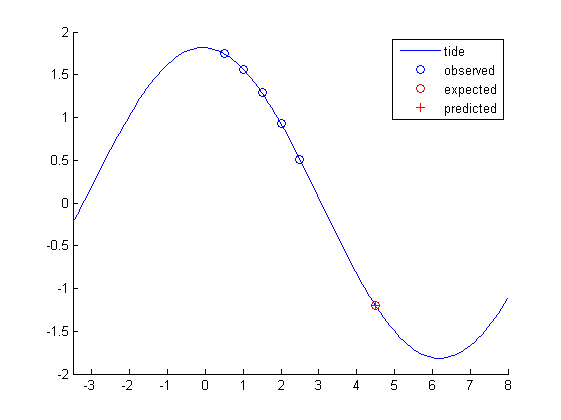
\includegraphics[width=0.6\textwidth]{simple_2h_1.png}
		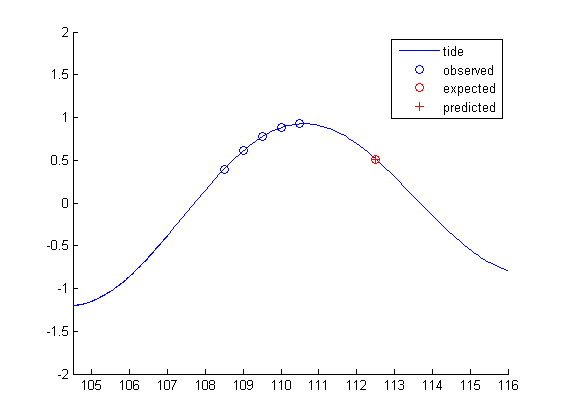
\includegraphics[width=0.6\textwidth]{simple_2h_2.png}
		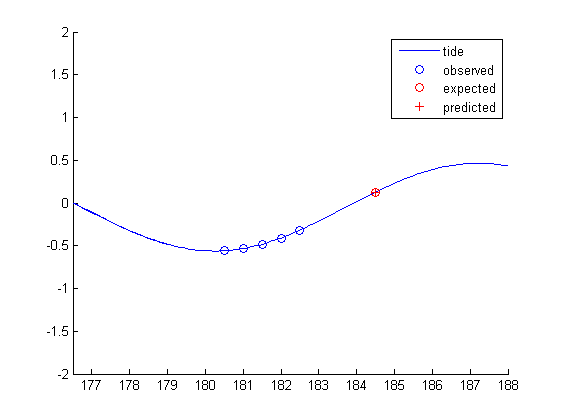
\includegraphics[width=0.6\textwidth]{simple_2h_3.png}
		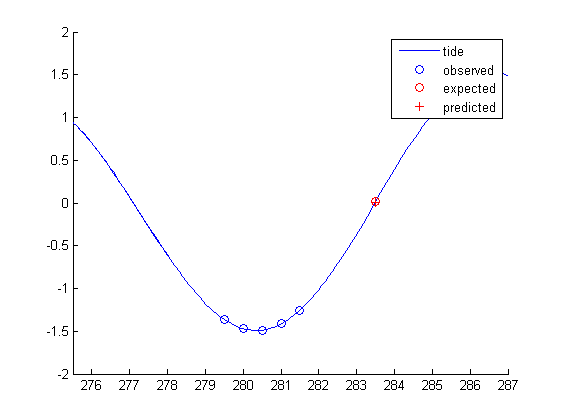
\includegraphics[width=0.6\textwidth]{simple_2h_4.png}
		\FloatBarrier
		
	\section{Predizione semplice massima}
		Per uno studio più approfondito dei limiti computazionali della rete lineare che simula il calcolo dell'altezza della marea si è provato quindi a determinare il numero massimo di ore di distanza dalla previsione, mantenendo lo scarto quadratico medio inferiore all'\textit{1\%}.\\
		\\
		Il risultato ottenuto, in via del tutto sperimentale, è di \textbf{36 ore} come intervallo massimo tra l'ultima marea osservata e la previsione che si vuole effettuare (osservando la marea ogni 2 ore) con un errore medio sull'altezza di marea inferiore all'\textbf{1\%}.
		Si noti che l'errore dell'\textit{1\%} risulta essere un valore molto basso, mentre \textit{36 ore} disponibili alla chiocciola per mettersi in salvo sul tronco di un albero sono più che sufficienti, per non dire eccessive: per errori più alti si può facilmente raggiungere un numero di ore per la previsione molto più alto, anche se inutile a fini pratici.\\
		\\
		Per riprodurre queste simulazioni basta impostare le variabili \textit{int} e \textit{forecast} a \textit{2} e \textit{36} rispettivamente (Codice \ref{lst:tideLin}).\\
		Di seguito alcuni grafici relativi a queste simulazioni:\\
		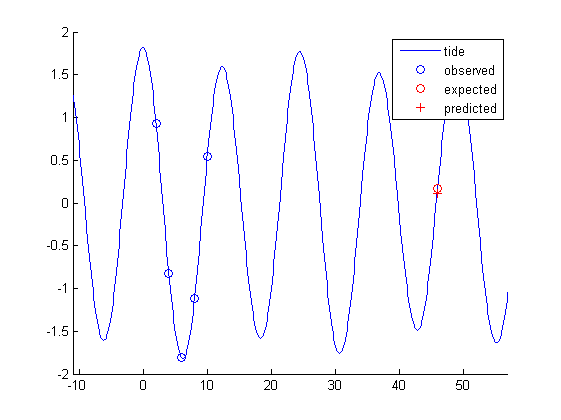
\includegraphics[width=0.6\textwidth]{simple_max_1.png}
		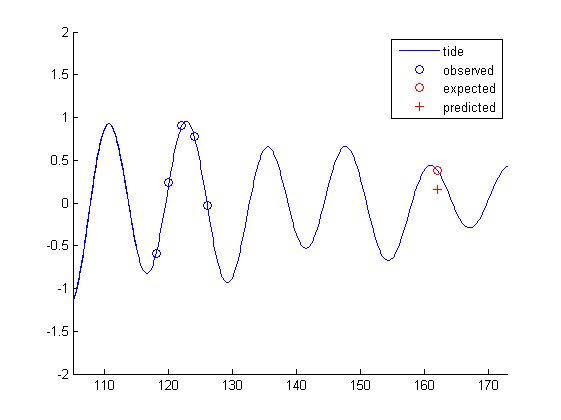
\includegraphics[width=0.6\textwidth]{simple_max_2.png}
		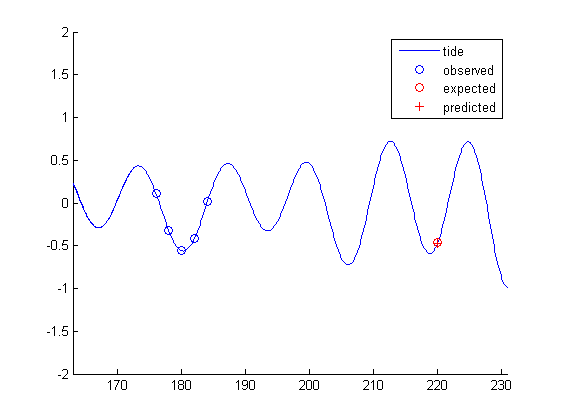
\includegraphics[width=0.6\textwidth]{simple_max_3.png}
		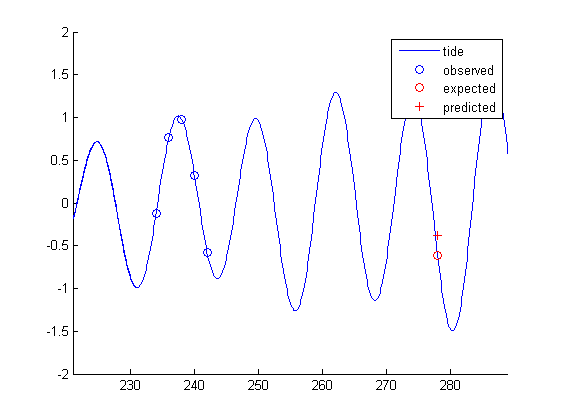
\includegraphics[width=0.6\textwidth]{simple_max_4.png}
		\FloatBarrier
	\chapter{Da AlViE ad HTML5}
	\label{chap:alvieHTML5}
	Concludiamo questo studio analizzando nel dettaglio come avviene l'esportazione delle visualizzazioni di AlViE in HTML5.\\
	\\
	Come abbiamo visto nel Capitolo \ref{chap:alvie}, AlViE memorizza le visualizzazioni in appositi file XML, che definiscono ogni singolo passo di visualizzazione. Inoltre, sia nel caso in cui l'utente voglia generare una nuova visualizzazione, sia che voglia caricarne una vecchia, il sistema disporr� del file XML corrispondente. Quindi, osservando che la struttura di un file XML e di un file HTML sono molto simili tra loro, per implementare l'esportazione della visualizzazione in HTML5 si � deciso di definire un opportuno compilatore da XML ad HTML5. Questo compilatore XML-HTML5 avr� quindi il compito di tradurre le specifiche della visualizzazione nel file XML in comandi Canvas nel file HTML5.
	\section{Specifica HTML5 delle visualizzazioni}
		Analizziamo innanzitutto come viene strutturata la pagina di visualizzazione HTML5.\\
		\\
		Innanzitutto troviamo, come in tutte le pagine HTML, il tag \lstinline{<html>} che racchiude tutto il codice, e pi� precisamente i tag \lstinline{<head>} e \lstinline{<body>}. Il tag \lstinline{<head>} contiene il tag \lstinline{<script language="Javascript">}, che definisce appunto uno script in JavaScript, suddiviso in una serie di funzioni. Il tag \lstinline{<body>}, invece, contiene la definizione del Canvas e dei quattro bottoni di navigazione, indicandone l'origine dell'immagine utilizzata, le dimensioni e la funzione JavaScript associata al click su ognuno di essi.\\
		Tramite l'attributo \lstinline{onLoad="start();"}, del tag \lstinline{<body>}, viene richiamata la funzione JavaScript \lstinline{start()}, che permette l'inizializzazione della visualizzazione, disegnando sulla pagina il primo step.\\
		\\
		Ad ogni passo dell'algoritmo corrisponde una funzione JavaScript, della forma
		\begin{center}
			\lstinline{function stepX()},
		\end{center}
		dove X rappresenta il numero del passo di visualizzazione. La funzione relativa al primo passo sar� quindi \lstinline{step0()}.\\
		A questo punto, tramite i quattro bottoni di navigazione in cima alla pagina, � possibile spostare la visualizzazione su un altro step. Al click di ogni bottone � associata una funzione JavaScript che calcola la funzione \lstinline{stepX()} da richiamare in base al numero di step attuale e al tipo di funzione richiamata. Le funzioni di navigazione sono quindi quattro, \lstinline{previous()}, \lstinline{next()}, \lstinline{first()} e \lstinline{last()}, che richiamano, rispettivamente, il passo precedente, il successivo, il primo o l'ultimo della visualizzazione. Nel caso in cui la visualizzazione sia sul primo step e venga richiamata la funzione \lstinline{previous()}, un messaggio d'errore verr� visualizzato dal browser; analogamente accadr� per l'ultimo step. Le quattro funzioni di navigazione si avvalgono della funzione \lstinline{eval(str)} per richiamare la giusta funzione di step: questa funzione prende come input una stringa \lstinline{str} e richiama la funzione corrispondente a tale stringa.\\
		\\
		Ogni funzione \lstinline{stepX()} dovr� quindi occuparsi, innanzitutto, di ripulire l'area del Canvas dal passo precedente, tramite la funzione \lstinline{contesto.clearRect(0, 0, canvas.width, canvas.height)}. Dopo aver ripulito l'intero Canvas, verranno richiamate opportune primitive grafiche per produrre il disegno vero e proprio, comprensivo di strutture dati, pseudocodice e messaggio.\\
		Viene anche definita una funzione \lstinline{writeMessage(contesto, messaggio, X)}, con X punto di partenza sull'asse delle ascisse, per poter disegnare sul Canvas il messaggio. � necessaria una funzione a s� stante, in quanto i messaggi pi� lunghi devono essere spezzati in pi� linee, che � appunto ci� di cui si occupa la funzione. In caso contrario, messaggi troppo lunghi produrrebbero un'area del Canvas esageratamente lunga, rendendone scomoda la lettura.
	\section{Compilatore XML-HTML5}
		Il compilatore XML-HTML5 che � stato scritto per questo progetto traduce linea per linea il contenuto del file XML della visualizzazione in comandi Canvas da scrivere nella pagina HTML. Vengono quindi aperti due stream (o flussi) dal sistema: uno in lettura dal file XML ed uno in scrittura sul file HTML. L'intero processo di traduzione del file XML della visualizzazione � divisibile in due fasi: una fase di parsing ed una fase di compilazione.\\
		\subsection{Fase di parsing}
			La prima fase, quella di parsing del file XML, consiste nell'analizzare il file XML della visualizzazione ed estrarne le informazioni contenute, organizzandole in oggetti dalla struttura nota e facilmente accessibili. In questo senso, sono stati analizzati, per questo studio, due diversi approcci per il parsing dei file XML: utilizzando un parser XML generico oppure utilizzando un parser scritto ad-hoc per la traduzione XML-HTML.\\
			\\
			Il parser XML generico utilizzato in questo studio � detto \textit{Digester}, ed � sviluppato e distribuito dalla Apache. Gli oggetti in cui archiviare le informazioni estratte dal file XML vengono invece detti \textit{Bean}. Appositi Digester si occuperanno di ogni tag incontrato, incapsulando le informazioni estratte in un oggetto Bean relativo al tag designato per il parsing. Ogni Digester dovr� essere inizializzato con apposite regole che gli indichino come estrarre e strutturare gli attributi di ogni tag incontrato. I Bean, poi, conterranno le informazioni estratte, fornendo anche metodi accessori per ottenere i valori dei vari attributi in un secondo momento.\\
			Gli oggetti Bean sono organizzati secondo una struttura gerarchica, rispecchiando l'organizzazione del file XML: ogni StepBean contiene, oltre ai suoi attributi, anche un insieme di StructureBean, relativi alle strutture contenute nel tag \lstinline{<step>}; analogamente ogni StructureBean conterr� il Bean del messaggio ed i Bean della struttura dati e della struttura dati grafica (ad esempio, ArrayBean e VisualArrayBean), e cos� via. L'insieme di tutti gli StepBean definisce, quindi, il file XML in modo completo, con tutte le informazioni in esso contenute ben organizzate e facilmente accessibili.\\
			\\
			Definendo, invece, un parser ad-hoc per l'esportazione di visualizzazioni AlViE in HTML, si ha che le informazioni ottenute  dal parsing dei vari tag non vengono archiviate in oggetti di tipo Bean, ma direttamente in vettori e variabili primitive, pronte per essere utilizzate ai fini della compilazione. Inoltre, la fase di parsing pu� essere fusa con quella di compilazione, alternando le due per ogni tag incontrato. Per contro, scrivere e maneggiare un parser ad-hoc � sicuramente pi� complesso rispetto all'utilizzo di un parser XML generico, scritto e testato da terzi.\\
			\\
			Comparando le due soluzioni su un calcolatore Netbook Packard Bell (CPU Intel Atom N280 @1.66 GHz, 1 GB di memoria RAM, Sistema Operativo Windows XP Home Edition SP3) si � potuto osservare che utilizzando il Digester come parser XML i tempi di compilazione raddoppiano rispetto alla soluzione ad-hoc. Questo � dovuto al fatto che la gestione del Digester stesso e degli oggetti Bean richiede sicuramente pi� risorse, rispetto alla gestione di qualche vettore. Inoltre, utilizzando il Digester � necessario dividere le fasi di parsing e di compilazione, eseguendo di fatto una compilazione in due passate (una per analizzare il file XML ed una per analizzare i Bean). Il parser ad-hoc viene invece fuso assieme al compilatore: ogni gestore di tag, come vedremo nella prossima Sesione, esegue il parsing del tag gestito ed utilizza subito le informazioni ottenute.\\
			A titolo d'esempio, eseguendo dei test sulla macchina sopra citata, l'algoritmo LCS (Longest Common Sequence), con una stringa di 10 caratteri ed una di 7 come input , richiede 3.6 secondi di compilazione con il parser ad-hoc, mentre ben 8.5 con il Digester. Analogamente, l'algoritmo di Dijkstra, eseguito su un grafo con 8 nodi, passa da 1 secondo di compilazione a circa 2.3 con il Digester.\\
			Si � quindi deciso di mantenere il parser ad-hoc, che permette al sistema di migliorare notevolmente le prestazioni in fase di compilazione XML-HTML5.
		\subsection{Fase di compilazione}
			Analizziamo quindi la compilazione vera e propria: ogni tag XML ha, all'interno del compilatore, una corrispettiva classe adibita alla gestione di quest'ultimo. Queste classi sono dette \textit{TagHandler}. Ogni volta che il compilatore si imbatte nell'apertura di un nuovo tag, viene invocata la classe \textit{TagHandlerFactory} la quale, implementando il design pattern del \textit{factory}, seleziona il giusto TagHandler per la gestione del tag.\\
			La gestione dei tag avviene quindi, da parte del compilatore, su pi� livelli, o gerarchie: gestori di livello superiore (o esterni) corrispondono ai tag pi� esterni del codice XML, come ad esempio \lstinline{<algorithm>} o \lstinline{<step>}; i gestori di livello inferiore corrispondono invece a quei tag situati all'interno di molti altri tag e che solitamente non ne contengono nessun altro, come \lstinline{<element>} o \lstinline{<node>}.\\
			\\
			Il gestore del tag \lstinline{<step>}, ad esempio, si occupa di definire la funzione \lstinline{stepX()} nel file HTML e inserire i comandi per la pulizia del Canvas. Quindi eseguir� un ciclo \textit{while} in cui invoca il TagHandlerFactory, finch� non si imbatte nella chiusura del tag \lstinline{<step>}, ovvero \lstinline{</step>}. Una volta usciti dal ciclo \textit{while}, e quindi raggiunta la chiusura del tag, il gestore si occuper� di scrivere le informazioni necessarie alla stampa del messaggio di step sul file HTML.\\
			\\
			I gestori dei tag di tipo \lstinline{<element>}, invece, non effettuano alcuna scrittura sul file, in quanto devono prima essere raccolte informazioni su tutti gli elementi di una struttura dati per avere informazioni sufficienti a poter disegnare quest'ultima. Il gestore di questo tipo di tag, quindi, si limita a passare le informazioni, raccolte dal parser, al gestore di livello superiore, che sar� il gestore di un tag di struttura, come \lstinline{<array>} o \lstinline{<matrix>}.\\
			Una volta ottenute le informazioni necessarie dai tag inferiori, il gestore del tag grafico della struttura (ad esempio \lstinline{<visualArray>}) avr� finalmente tutte le informazioni necessarie per ricavare le primitive grafiche che produrranno il disegno nella pagina HTML.\\
			Spesso per�, le informazioni raccolte dai singoli elementi non definiscono in maniera esplicita le operazioni grafiche necessarie. Nella specifica XML di un vettore, ad esempio, vengono indicate le coordinate d'origine dell'intero vettore, non di ogni singolo elemento. Tutti questi dati, \textit{impliciti} nella specifica XML, dovranno quindi essere calcolati, tramite apposite funzioni, per poter disegnare nella pagina i singoli elementi grafici che compongono il disegno finale.
		\subsection{Pesantezza della pagina vs. pesantezza di compilazione}
			Ha senso, a questo punto, domandarsi a chi spetta l'onere di calcolare tutti questi dati impliciti. Le scelte sono chiaramente due: il calcolo pu� essere fatto \textit{a monte}, ovvero dal compilatore, oppure \textit{a valle}, cio� dal browser HTML che visualizza la pagina.\\
			\\
			Se viene scelto di effettuare questi calcoli lato browser, si avr� sicuramente una compilazione pi� veloce. Il compito del browser verr�, invece, appesantito, rendendosi necessaria l'occupazione di risorse per il calcolo di questi dati impliciti. Questo approccio permette, tuttavia, di riutilizzare il codice necessario alla visualizzazione di stessi oggetti grafici. Pu�, ad esempio, essere definita una funzione che disegni un quadrato, una che disegni un vettore o una che disegni un intero grafo. Se in una visualizzazione appaiono, ad esempio, pi� vettori, la visualizzazione di ogni nuovo vettore si tradurr�, nella pagina HTML, in un'unica invocazione della funzione adibita a disegnare vettori.\\
			Quindi questa scelta velocizza il compilatore, rallenta il browser e alleggerisce la pagina.\\
			\\
			Scegliere, invece, di effettuare i calcoli \textit{a monte} implica, chiaramente, un maggior costo computazionale del processo di compilazione. D'altro canto, la pagina HTML verr� alleggerita, per quanto riguarda il costo computazionale, in quanto il compilatore potr� scrivervi direttamente le primitive grafiche necessarie, senza bisogno di ulteriori calcoli. Tuttavia, utilizzare primitive grafiche, all'interno della pagina HTML, significa essere costretti a ripetere il codice necessario al disegno di uno stesso oggetto. Se la visualizzazione deve, ad esempio, disegnare pi� vettori, ognuno dei quali disegnato da (indicativamente) 10 primitive grafiche, si avranno nella pagina HTML 10 linee di codice per ogni nuovo vettore da visualizzare. Si vede che, rispetto al caso precedente, le dimensioni della pagina risultano aumentate di circa un fattore $m$, dove con $m$ si indica il numero medio di primitive necessarie alla visualizzazione di un oggetto grafico elementare.\\
			Riassumendo: questa scelta ci porta ad una compilazione pi� lenta, una visualizzazione pi� veloce ed una pagina Web pi� pesante.\\
			\\
			Non esiste, come si pu� vedere, una scelta ottimale: le due strade presentano sia pregi che difetti. Quale scelta intraprendere dipende allora dal tipo di applicazione per cui si � reso necessario il compilatore.\\
			Nel nostro caso, ovvero la visualizzazione di algoritmi sul Web, si � ritenuto pi� efficiente optare per i calcoli dei dati \textit{a monte}. Si � ipotizzato, infatti, che siano di pi� le volte in cui una visualizzazione viene eseguita (ovvero visualizzare i vari step che la compongono), rispetto alle volte in cui essa viene creata (tramite il compilatore) o caricata tramite Internet. Le dimensioni della pagina HTML sono infatti inversamente proporzionali al tempo necessario per il suo download.\\
			Ricapitolando, abbiamo optato, durante lo sviluppo di questo progetto, per una compilazione ed un tempo di download della pagina pi� lenti, a favore di visualizzazioni pi� rapide. Questo dilemma risulta, tuttavia, puramente teorico: nella pratica, la scelta di questo metodo al posto dell'altro si riduce ad una manciata di KB in pi� nella dimensione delle pagine e a pochi millisecondi in pi� di compilazione. Anche la velocit� di visualizzazione da parte del browser risulta praticamente identica. Quindi la scelta � stata presa a livello puramente teorico, in quanto a livello pratico i due metodi sono di fatto indistinguibili.\\
			\\
			Mostriamo, a titolo d'esempio, la funzione che calcola le primitive per il disegno di un cerchio, definita all'interno del compilatore di AlViE:
			\lstinputlisting[language=java]{code/circle.java}
			Si pu� vedere, in quest'esempio, che il compilatore si occupa di calcolare alcuni dettagli, come il raggio del cerchio o la dimensione del testo all'interno, per poi scrivere sulla pagina HTML le primitive grafiche corrispondenti, come \lstinline{ctx.arc()}.
	\chapter*{Conclusioni}
	\addcontentsline{toc}{chapter}{Conclusioni}
	Concludiamo questo studio con alcune considerazioni generali su quanto trattato.\\
	\\
	La quarta versione di AlViE, nata sulla base delle nuove funzioni implementate nel corso di questo lavoro, risulta essere molto in avanti rispetto alla versione precedente: il supporto al Web permette la condivisione su larga scala delle visualizzazioni generate, facilmente inseribili in un qualsiasi sito Web. All'interno del libro di testo Strutture di Dati e Algoritmi (seconda edizione; Pierluigi Crescenzi, Giorgio Gambosi, Roberto Grossi, Gianluca Rossi; Pearson) sono gi� state utilizzate, a scopo didattico, diverse visualizzazioni prodotte con AlViE. Inoltre, sul sito Web di suddetto libro (http://wps.pearsoned.it/crescenzi\_strutture-dati-algoritmi2/220/56566/14480998.cw/index.html) si possono trovare alcune visualizzazioni di AlViE esportate come pagina HTML, ai fini di supportare lo studio e la comprensione delle principali strutture ed algoritmi.\\
	L'editor di strutture dati, invece, aggiunge un nuovo livello d'interazione utente-sistema, facilitando la specifica degli input. Con questa nuova versione vengono anche alleggerite le conoscenze richieste all'utente che voglia definire la propria visualizzazione: adesso, infatti, non � pi� richiesto in alcun modo che l'utente capisca e gestisca la specifica XML delle strutture dati, che saranno completamente occultate agli occhi di quest'ultimo.\\
	\\
	AlViE si sta quindi avviando verso una maggior accessibilit� e semplicit� d'utilizzo, dimostrando di avere buone probabilit� di inserirsi nel contesto mondiale dei sistemi di visualizzazione di algoritmi, tenendo testa ai maggiori esponenti del settore, come JHAV� o OpenDSA.\\
	\\
	Concludendo, il lavoro svolto, dalla costruzione del compilatore e dell'editor di testo, allo studio dell'universo dei sistemi di visualizzazione di algoritmi, si � dimostrato essere molto interessante, a livello sia pedagogico che personale. Questo lavoro � riuscito, infatti, a conciliare pratica e teoria, nel campo della visualizzazione di algoritmi, e, pi� in  generale, dell'Informatica.
	
	\nocite{*}
	\bibliographystyle{plainnat}
	\bibliography{bibliography}

\end{document}